\chapter{Results}\label{chap:results}

    In this chapter I will show results of my calculations. I start from the deuteron photodisintegraion process
    (Section~\ref{sec:de_results}),
    presenting predictions and discussing the cross (subsection~\ref{sec:cross_results}) 
    and polarization observables  (subsection~\ref{sec:polarisation_results}).Next, in 
    Section~\ref{sec:hel_results} I will present my predictions of the observables
    for $^3$He photodisintegration.
    \tmp{...}
    Finaly in Section~\ref{sec:pion_results} I will discuss results of the calculations
    for pion absorption from the lowest atomic orbital.

\section{Deuteron photodisintegraion}
\label{sec:de_results}
    \subsection{Cross section}
    \label{sec:cross_results}

    In this section I will show the results of my calculation starting from the
    deuteron photodisintegration process. One of the most
    studying observable is obviously the cross section. There is
    a number of papers which present 
    measurement results for both differential and total cross section
    \cite{BOSMAN1979,ARENDS1984,Skopik1974, Moreh1989, Birenbaum1985, Bernabei1986, rachek2007,Ying_Experiment_Deut, DeSanctis_Experiment_Deut} 
    and it seems interesting to compare 
    our predictions with experimental results.

    In Fig.~\ref{TOTAL_CROSS_small} and Fig.~\ref{TOTAL_CROSS} 
    I present predictions for the
    total cross section $\sigma_{tot}~[\mu\text{b}]$ which I obtained
    using the chiral \gls{sms} potential at the N$^4$LO+ order and with 
    the cutoff parameter $\Lambda=\SI{450}{\mev}$.
    From Fig.~\ref{TOTAL_CROSS_small}, we see that at low photon energies
    (below 50 MeV) predictions which include 2N contributions
    to the electromagnetic current
    via the Siegert approach, describe experimental results quite well.
    We can suppose that the difference with experimental data may come from 
    the statistical uncertainty of  the data itself, as my predictions
    are often in between the data from different experiments.
    Moreover, even at such low energies the 1N current is clearly not enough
    to describe cross section - dashed pink line has much lower values and
    the difference becomes even larger with increasing photon energies.
    At 5~MeV the difference between 1N predictions
    and 1N + Siegert is 297.54~$\mu$b (10.8\%), increasing energy to 10 MeV
    it is 304.28~$\mu$b (20.4\%) and at 20~MeV it is 229.50~$\mu$b (39.2\%).
    % Even with energy increasing from 5~MeV to 20~MeV -
    % the difference between predictions has changed from 10.8\% to 39.2\% and
    From \fig{TOTAL_CROSS_small} we see that the gap between these predictions
     continues increasing even more with larger energies.
    This tells us that Siegert approach works quite well as no additional 2N contributions are taken into account.
    The cross section predictions corrected via Siegert 2N contribution  reproduce 
    experimental data to some extend.

    Here and later the relative difference between set of predictions ($x_1$, $x_2$, ..., $x_N$) is calculated
    using the formula:

    \begin{equation}
        \Delta = \frac{\max(x) - \min(x)}{\frac{1}{N}\sum_{i=1}^N x_i} \cdot 100\%,
        \label{eq:relative_diff}
    \end{equation}
    so in the specific case of comparison the date with 1N current and "1N + Siegert" we
    calculate relative difference as 
    $\Delta = \frac{|\sigma^{1N+Siegert} - \sigma^{1N}|}{0.5(\sigma^{1N+Siegert} + \sigma^{1N})}$.

    While my main goal is to describe deuteron photodisintegration at low energies, 
    where predictions seem to be well describing experimental data at
    $E_\gamma \lesssim \SI{50}{\mev}$, it is also interesting to check how 
    present theory works at higher energies.
    At the higher energies (above $E_\gamma=\SI{50}{\mev}$, Fig.~\ref{TOTAL_CROSS})
    we can notice that the discrepancy with experimental data is not only 
    quantitative, but also qualitative.  
    This starts already above $E_\gamma=\SI{50}{\mev}$ and is especially pronounced at peak around \SI{300}{\mev}
    seen in the experimental data from \cite{Bernabei1986} which is not
    reflected in predictions. The reason of such discrepancy 
    is most likely coming from the relativistic effects
    which we do not take into account within this work.
    It is also confirmed by the calculations in \cite{ArenhovelPhotodisint1991}
    where authors discuss different potentials applying to the deuteron photodisintegration.
    Despite authors use a much simpler potentials that used in this thesis, their predictions obtained with including
    some relativistic effects show, that such a peak appears in predictions. 
    
    
     The higher energies region is presented in order
    to investigate how far the predictions are from experimental results and 
    what should be improved in the future (e.g. include relativistic part). 
    
    \begin{figure}[h]
        \begin{center}
        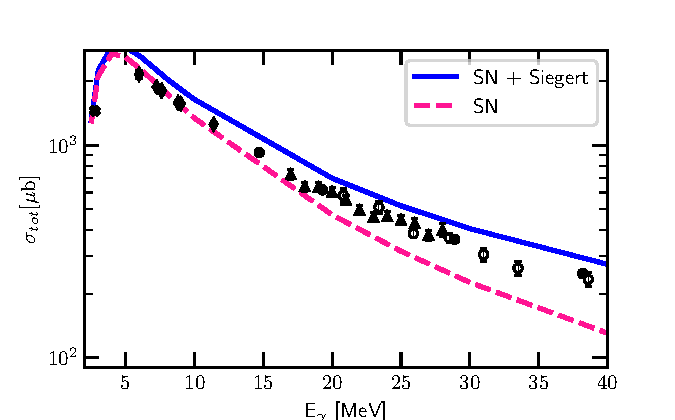
\includegraphics[width=0.75\textwidth]{Figures_De/TOTAL_CROSSSECTION_SMALL_REGION.pdf}
        \end{center}
        \caption{Total cross section $\sigma_{tot}$ for the deuteron photodisintegration process
        as a function of the photon's energy E$_\gamma$.
        Solid blue line presents results obtained with SN+Siegert 
        and dashed pink line - predictions based on the SN current.
        In both cases the \gls{sms} N$^4$LO+ $\Lambda=\SI{450}{\mev}$ force is used.
        The experimental data are from \cite{Bernabei1986} (black filled circles),
        \cite{BOSMAN1979} (empty circles),
        % \cite{ARENDS1984} (squares),
        \cite{Skopik1974} (triangles),
        \cite{Moreh1989} (bold cross "X") and
        \cite{Birenbaum1985} (diamonds).
        }
        \label{TOTAL_CROSS_small}
    \end{figure}

    
    \begin{figure}[htb!]
        \begin{center}
        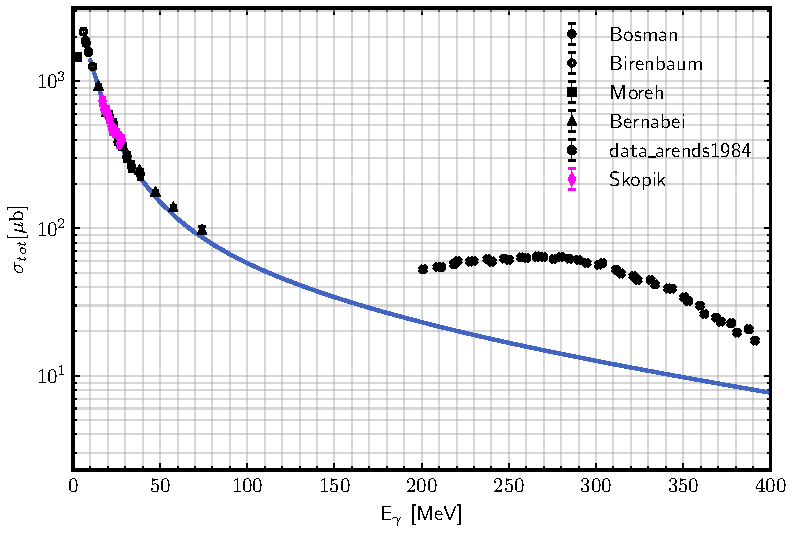
\includegraphics[width=0.75\textwidth]{Figures_De/TOTAL_CROSSSECTION.pdf}
        \end{center}
        \caption{The same as in \fig{TOTAL_CROSS} but for the energy range 2.5 - 400 MeV.
        The experimental data are the same plus data above $E_\gamma=\SI{200}{\mev}$ from
        \cite{ARENDS1984} (crosses).
        }
        \label{TOTAL_CROSS}
    \end{figure}

    \begin{figure}[htb!]
        \begin{center}
            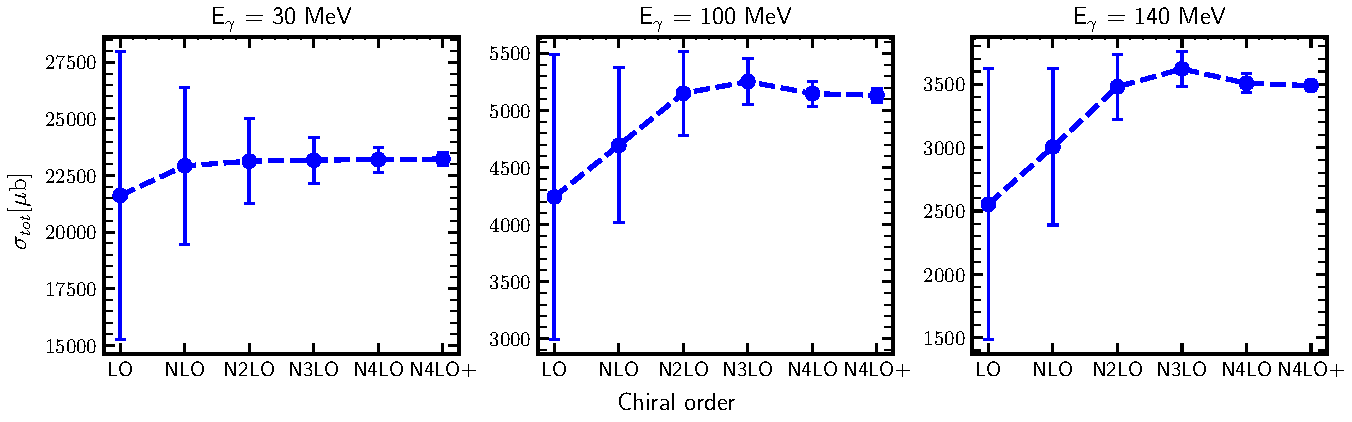
\includegraphics[width=0.95\textwidth]{Figures_De/TOTAL_CROSSSECTION_Truncation.pdf}
        \end{center}
        \caption{Total cross section of the deuteron photonisintegration
        process as a dependance on the chiral order for three photon energy E$_\gamma$ values: \SIlist[list-units = single]{30;100;140}{\mev}.
        Error bands show an estimated truncation error at each order.}
        \label{Trunc_100}
    \end{figure}
    
    In Fig. \ref{Trunc_100} I present the
    total cross-section for the deuteron photodisintegration 
    at three photon energy values: \SIlist[list-units = single]{30;100;140}{\mev} as a function of the chiral order.
    Error bands show truncation errors calculated using Eq.~\ref{trunc2}~-~\ref{trunc5}.
    One can see that truncation errors are being reduced with each consecutive chiral order. 
    At LO it is the biggest: \SI{29.46}{\percent} at $E_\gamma = \SI{30}{\mev}$,
    \SI{29.46}{\percent} at $E_\gamma = \SI{100}{\mev}$ and
    \SI{41.82}{\percent} at $E_\gamma = \SI{140}{\mev}$.
    At N4LO+ it is hardly visible at presented scale and amounts up to 
    \SI{1.3}{\percent} for each energy.
    For each energy the prediction is within the uncertainty range of lower orders.
    We see that at lower energy $\sigma_{tot}$ already at NLO reaches valve which remains
    practically unchanged at higher orders.
    Contrary, at two higher energies, contributions from higher orders are necessary to obtain 
    stable predictions 

        
    Figures \ref{Diff_cross_order_pw} and \ref{Diff_cross_err} show my predictions 
    for the differential cross section
    $\frac{d\sigma}{d\Omega}$.
    In both figures the top, middle and bottom row shows predictions at 
    $E_\gamma = \SIlist[list-units = single]{30;100;140}{\mev}$, respectively.
    with 2N current's contributions taken into account via Siegert theorem.
    If not stated otherwise I use th \gls{sms} N$^4$LO+ potential.
    % They all are organized in a similar way: the left panel
    % presents predictions obtained using \gls*{sms} potential at different chiral orders (from LO to N$^4$LO+)
    % with cutoff parameter $L = \SI{450}{\mev}$,
    % the middle panel includes the truncation error's bands (described in Sec. \ref{sec:deut_bound})
    % for each chiral order starting
    % from NLO. And the right panel shows predictions obtained with different values of the
    % cutoff parameter at the chiral order N$^4$LO+.
    The left column of \fig{Diff_cross_order_pw} shows the predictions obtained at 
    different chiral orders (from LO to N$^4$LO+) and with $\Lambda=\SI{450}{\mev}$.
    Looking at the best predictions (N$^4$LO+, $\Lambda=$~\SI{450}{\mev}) for each
    energy, I
    conclude that the higher photon's energy is, the larger is 
    difference between the theoretical predictions and experimental 
    data. At $E_\gamma = \SI{30}{\mev}$ (top panel) my predictions
    almost perfectly match the data and the difference is almost always
    within the experimental uncertainties. 
    Moving to  $E_\gamma=\SI{100}{\mev}$ (middle row)
    the description of the data is deteriorating: theoretical
    predictions still match the data qualitatively, but
    the gap for proton emission angle $\theta_p$ in range ($\ang{60} < \theta_p < \ang{130}$) 
    is up to \SI{32}{\percent} (of the predicted value) and relative difference is up to
    \SI{7}{\percent} (calculated with \eq{eq:relative_diff}).
    At the highest energy(bottom figure), it is even hard to say about 
    good qualitative description: the general trend of the
    angular dependance is presented, but the predictions are 
    far from the experimental points.
    We observe improvements introduced by each subsequent chiral order, but 
    stabilization shows that some ingredients are missing.

    Obtained results at each energy confirm the convergence 
    of the predictions with respect to the chiral order.
    We see that the cross section at LO is far from both experimental 
    data and the best potential's predictions (N$^4$LO+) and
    the higher photon's energy, the larger is this
    difference. With each subsequent chiral order, the 
    curves are more closer to each other and the difference
    between N$^4$LO and N$^4$LO+ is hardly visible at scale used in \fig{Trunc_100}.
    The relative difference between these two predictions at $E_\gamma=\SI{30}{\mev}$ around the point of maximum 
    ($\theta_p = \ang{80}$) is \SI{0.05}{\percent} which is \SI{0.02}{\micro \barn \per \steradian};
    at \SI{100}{\mev} and $\theta_p = \ang{107}$ it is \SI{0.79}{\percent} (\SI{0.025}{\micro \barn \per \steradian});
    and at \SI{140}{\mev} (same angle) it is \SI{1.8}{\percent} (\SI{0.043}{\micro \barn \per \steradian}).
    Having such a small differences between predictions from two highest chiral orders,
    I can conclude that predictions are converged and 
    using NN potential at subsequent chiral orders would rather not bring large contribution 
    to the cross section values. 
    The difference with experimental data is rather systematic 
    and is independent on the chiral order. 
    The relative difference between experimental data and predictions obtained with $N^4LO+$ and $\Lambda=$~\SI{450}{\mev} at \SI{30}{\mev} is less then \SI{13}{\percent}
    and absulute difference is < \SI{3.07}{\micro \barn \per \steradian}.
    At \SI{100}{\mev} descripancy is larger and relative difference reaches 46\% with absolute difference up to \SI{1.39}{\micro \barn \per \steradian}.
    Coming to \SI{140}{\mev} the relative difference 
    increases up to \SI{48.6}{\percent} and absolute - \SI{1.93}{\micro \barn \per \steradian}.
    What may be helpful
    for a better data description is a 2N current 
    and relativistic correction, mentioned earlier.

    Predictions obtained with \gls*{av18} potential (dashed-dotted purple line on the \fig{Diff_cross_order}) show that
    it is very similar at lower energies (relative difference at \SI{30}{\mev} is \SI{0.06}{\percent}
    at the point of maximum - \ang{80}) and with increasing energy to \SI{140}{\mev}
    it growes to \SI{3.1}{\percent]} at same angle. 
    It can be connected with our potential's quality loss, but \gls*{av18} can
    be struggling with high energies as well.

    The Fig.~\ref{Diff_cross_truncation} 
    presents theoretical truncation uncertainties and it once more
    confirms that for the regarded nuclear reaction chiral order
    N$^4$LO+ is able to produce converged predictions: 
    the black band is hardly visible for the $E_\gamma=$~\SI{30}{\mev}
    (the relative error for N$^4$LO+ at \ang{80} is only \SI{0.12}{\percent})
    and is also quite narrow for larger energies (at \SI{140}{\mev} 
    the error at the same angle is \SI{1.42}{\percent}). 

    Fig.~\ref{Diff_cross_cutoff} presents a cutoff dependency
    of predictions. The ideal case is when the dependency is so weak that
    the choice of the parameter $\Lambda$ would not make large 
    changes. In practice the choice of this parameter can be 
    important as it makes a noticeable difference in predictions.
    
    On the top of \fig{Diff_cross_cutoff} (when $E_\gamma=$~\SI{30}{\mev}) the cutoff dependance is so weak,
    that, in fact, all the lines (for different $\Lambda$ values)
    overlap each other and we cannot distinguish them with the naked eye:
    the relative difference ar maximum is \SI{0.08}{\percent}.
    Nevertheless, with increasing photon's energy to \SIlist{100; 140}{\mev} 
    (middle and bottom rows of \fig{Diff_cross_cutoff}) the spread becomes larger:
    the cutoff error is  \SI{3.35}{\percent} at \SI{100}{\mev}
    and \SI{5.56}{\percent} at \SI{140}{\mev} (the same $\theta_p$). 

    On the Fig.~\ref{Cutoff_dep} we saw that the total
    cross section for the same energies has the cutoff spread
    around \SI{4.5}{\percent} for \SI{100}{\mev} and \SI{8}{\percent} for \SI{140}{\mev}. For \SI{30}{\mev} it is below  \SI{1}{\percent}.
    
    In \fig{Diff_cross_pw_1nc} I show different components of the best prediction (N$^4$LO+, $\Lambda=\SI{450}{\mev}$)
    for three values of photon's energy. Prediction with plane-wave component only (without rescattering part)
    has relatively small deviation from the full predictions, but the difference increases at larger energies.
    With $E_\gamma=\SI{30}{\mev}$ the relative difference is \SI{10}{\percent} (\SI{4.03}{\micro \barn \per \steradian})
    at $\theta_p = \ang{80}$. Difference at \SI{100}{\mev} and the same angle is \SI{4}{\percent} (\SI{0.21}{\micro \barn \per \steradian})
    and at \SI{140}{\mev} it is \SI{7}{\percent} (\SI{0.21}{\micro \barn \per \steradian}).
    In contrast, predictions without Siegert component (1NC) have much larger gap with full prediction:
    the difference is \SI{46.5}{\percent} (\SI{13.67}{\micro \barn \per \steradian}) at \SI{30}{\mev},
    \SI{78.6}{\percent} (\SI{2.88}{\micro \barn \per \steradian}) at \SI{100}{\mev} and
    \SI{77.8}{\percent} (\SI{1.68}{\micro \barn \per \steradian}) at \SI{140}{\mev}.
    Obviously 2NC contributions are extremely important in this case, the difference connected with 2NC
    contributions is much higher then theoretical errors or even rescattering contribution.



    \begin{figure}[h]
        \centering
        \begin{subfigure}[t]{0.46\textwidth}
            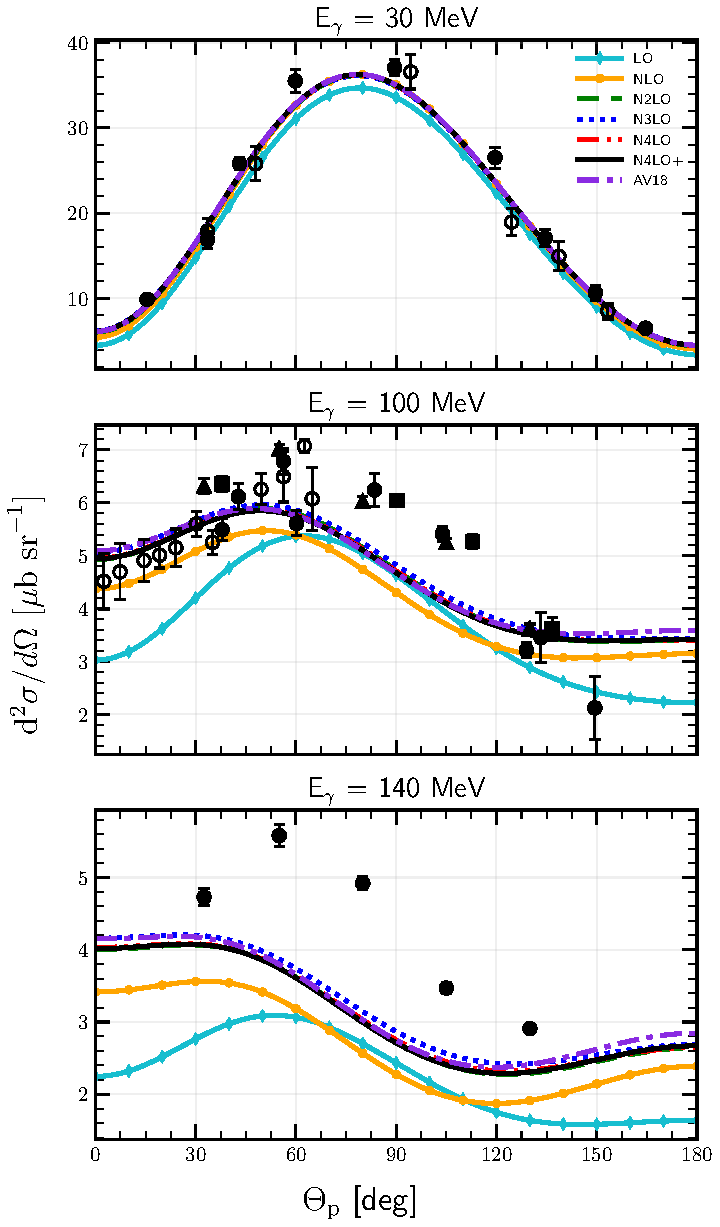
\includegraphics[width=\textwidth]{Figures_De/CROSS2_order_vert.pdf}
            \caption{}
            \label{Diff_cross_order}
        \end{subfigure}
        \begin{subfigure}[t]{0.46\textwidth}
            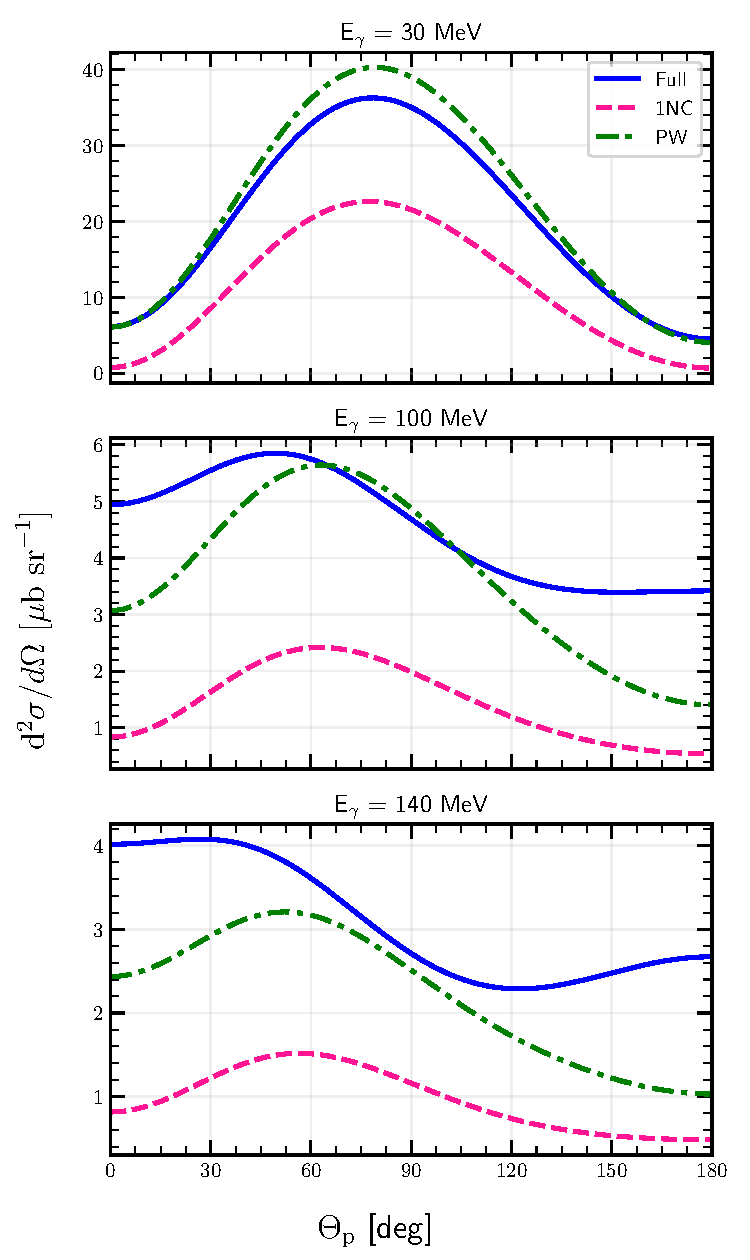
\includegraphics[width=\textwidth]{Figures_De/Diff_cross_pw_1nc.pdf}
            \caption{}
            \label{Diff_cross_pw_1nc}
        \end{subfigure}
        \caption{Differential cross section as a function of the outgoing proton angle in the center of mass frame 
        for the photon's energy \SI{30}{\mev} (top), \SI{100}{\mev} (middle) and \SI{140}{\mev} (bottom).
        {\bf (a)} Results obtained using \gls*{sms} potential
        at different chiral orders (from LO to N$^4$LO+) with the cutoff parameter $\Lambda=\SI{450}{\mev}$ and 
        2NC contributions taking via Siegert theorem.
        For the sake of comparison, predictions obtained with the \gls*{av18} potential are on both figures as well.
        Data points (filled and empty circles) are from \cite{Ying_Experiment_Deut}
        for $E_\gamma=\SIlist[list-units = single]{30; 100}{\mev}$
        and \cite{DeSanctis_Experiment_Deut} for $E_\gamma=\SI{140}{\mev}$.
        {\bf (b)} Predictions obtained with chiral N$^4$LO+ potential and $\Lambda=\SI{450}{\mev}$.
        Blue solid line is a best predictions we have (plane-wave plus rescattering parts, 1NC + Siegert), pink dashed line shows predictions obtained with
        single-nucleon current only (without Siegert contributions) and green dashed-dotted line
        is a prediction with plane-wave part only - without rescattering.
        }
        % Results in {\bf (a)} are obtained using \gls*{sms} potential
        % at different chiral orders (from LO to N$^4$LO+) with the cutoff parameter $\Lambda=\SI{450}{\mev}$ and 
        % 2NC contributions taking via Siegert theorem.
        % Data points (filled and empty circles) are from \cite{Ying_Experiment_Deut}
        % for (\SIlist[list-units = single]{30; 100}{\mev})
        % and \cite{DeSanctis_Experiment_Deut} (for energy \SI{140}{\mev}).
        % Predictions obtained with chiral N$^4$LO+ potential and $\Lambda=\SI{450}{\mev}$ are on {\bf (b)}.
        % Blue solid line is a best predictions we have (plane-wave plus rescattering parts, 1NC + Siegert), pink dashed line shows predictions obtained with
        % single-nucleon current only (without Siegert contributions) and green dashed-dotted line
        % is a prediction with plane-wave part only - without rescattering.}
        \label{Diff_cross_order_pw}
    \end{figure}


        
    \begin{figure}[h]
        \centering
        \begin{subfigure}[t]{0.46\textwidth}
            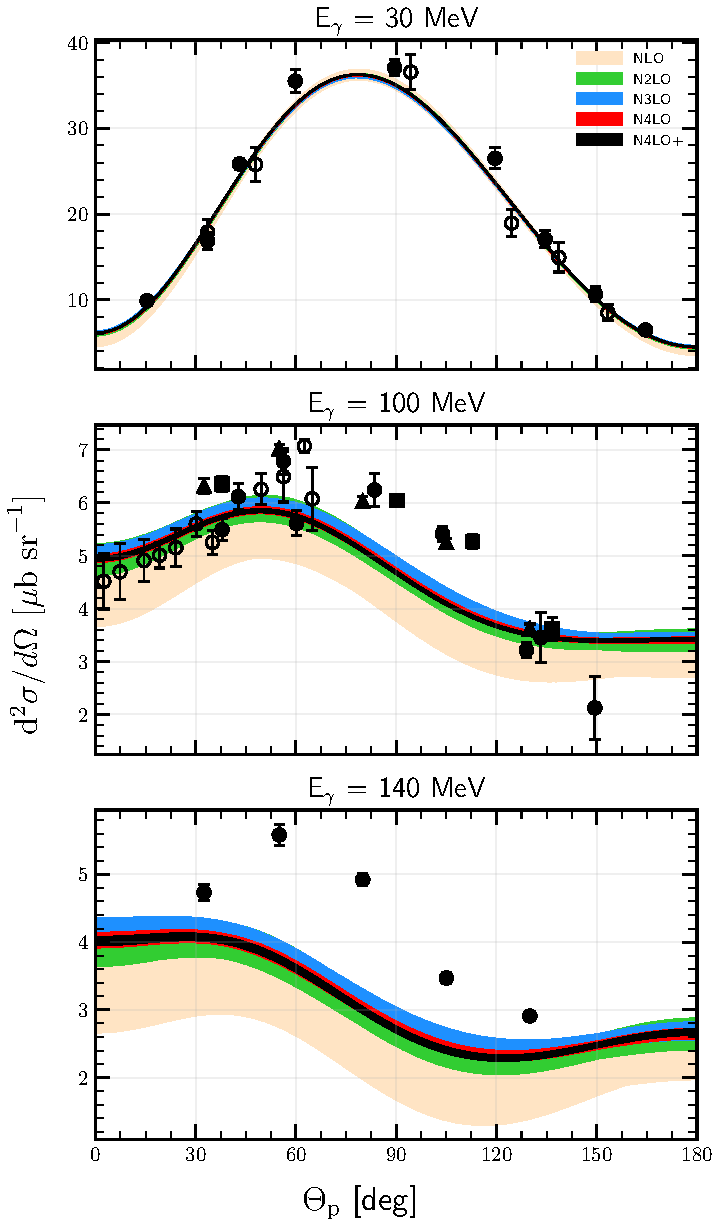
\includegraphics[width=\textwidth]{Figures_De/CROSS2_truncation_vert.pdf}
            \caption{ Truncation error bands.}
            \label{Diff_cross_truncation}
        \end{subfigure}
        \begin{subfigure}[t]{0.46\textwidth}
            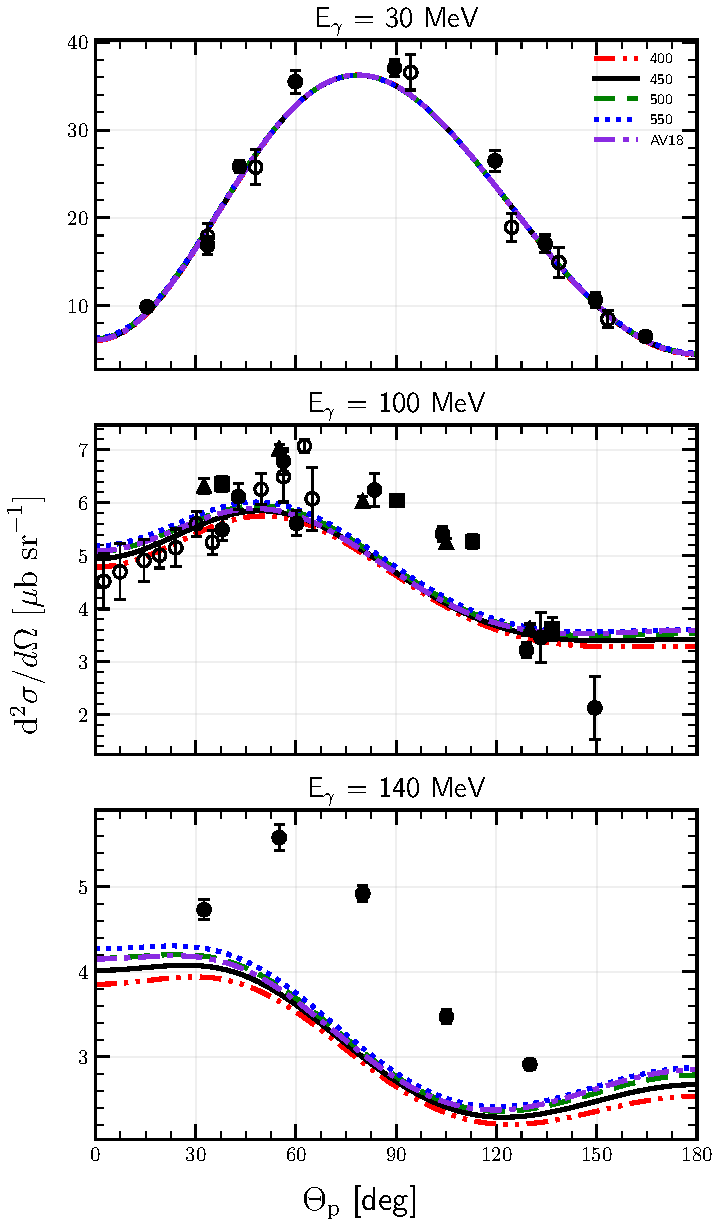
\includegraphics[width=\textwidth]{Figures_De/CROSS2_cutoff_vert.pdf}
            \caption{Cutoff dependance  of predictions.}
            \label{Diff_cross_cutoff}
        \end{subfigure}
        \caption{Theoretical uncertainies 
        for the differential cross section $\frac{d^2\sigma}{d\Omega}$
        as a function of the outgoing proton's momentum polar angle $\theta_p$ in the center of mass frame 
        for the photon's energy is \SI{30}{\mev} (top row), \SI{100}{\mev} (middle row) and \SI{140}{\mev} (bottom row).
        {\bf(a)} The truncation error bands for each energy in a corresponding row. 
        Results are obtained using potential with different chiral orders (from NLO to N$^4$LO+) 
        with cutoff parameter $\Lambda=\SI{450}{\mev}$ and 2NC contributions taking via Siegert approach.
        {\bf (b)} Predictions obtained using different values of the cutoff parameter $\Lambda$
        (double-dotted-dashed red line presents results obtaining with 
        a cutoff values $\Lambda=\SI{400}{\mev}$, solid black line - \SI{450}{\mev}, dashed green line - \SI{500}{\mev}
        and dotted blues line - \SI{550}{\mev}) and the chiral potential N$^4$LO+. 
        Data points are the same as in \fig{Diff_cross_order}}
        \label{Diff_cross_err}
    \end{figure}

    \clearpage

    \subsection{Polarisation observables}
    \label{sec:polarisation_results}

    In this subsection I will present my predictions for 
    selected polarisation observables.
    I start with deuteron analyzing power $T_{20}$, $T_{21}$ and $T_{22}$,
    which according to \cite{ArenhovelPhotodisint1991} are defined as:
    
    \begin{equation}
        T_{2i} (\theta) = \frac{(2 - \delta_{i0}) \Re V_{2i}}{V_{00}}, i=0,1,2
    \end{equation}

    On the Figures \ref{T20_T21_30} (a, b) and \ref{T22_T11_30}(a,b)
    I show my predictions for the
    $T_{20}$, $T_{21}$,  and $iT_{11}$ respectively as a functions 
    of the outgoing proton angle $\theta$ in the CM frame. Each of them
    is prepared with photon's energy 30~MeV and is
    organized in the similar way: the top
    pane shows a dependance of the predictions on the 
    chiral order of the potentia. The middle subfigure is
    showing a correspondent truncation error for each of the 
    predictions from a top one (without LO, because its uncertainty is
    too large and will make the readability worse). The last (bottom)
    pane shows the cutoff dependance for each observable at the chiral
    order N$^4$LO+. 

    All the polarisation observables presented here, show a good convergence 
    upon a chiral order as it is hard to distinguish the predictions
    from each subsequent order starting from the N$^2$LO.
    The relative width of N$^4$LO+ truncation band 
    for T$_{20}$, T$_{21}$ and T$_{22}$
    are \SIlist{0.06; 0.05; 0.19}{\percent} respectively (at $\theta_p=$ \ang{90}, \ang{60} and \ang{90} respectively).
    The slowest convergence is observed for $iT_{11}$ (Fig.~\ref{T11_30_vert})
    where we can stll recognize N$^2$LO band.
    Still it has only a \SI{0.2}{\percent}
    width of N$^4$LO+ truncation band at $\theta_p = \ang{20}$ (maximum point).
    The cutoff dependency for all regarded observables is weak and 
    predictions for each value of the $\Lambda$ are hardly separable 
    with the naked eye.
    The relative spread of cutoff predictions at the same angles as above 
    are \SIlist{0.87; 0.94; 3.42; 0.68}{\percent} respectively for T$_{20}$, T$_{21}$, T$_{22}$ and $i\text{T}_{11}$ respectively.


    Predictions for the photon's energy $E_\gamma = \SI{100}{\mev}$
    (Figs. \ref{T20_T21_100} and \ref{T22_T11_100}) preserve similar
    trends for each obserable. 
    Generally, predictions are being converged starting
    even from the N$^2$LO while for $iT_{11}$
    we can see 
    that truncation error's bands are noticeably wide
    even at N$^4$LO and N$^4$LO+
    Cutoff dependance at this energy is a bit stronger, especially
    for 
    $T_{22}$ and $iT_{11}$ components (Fig.~\ref{T22_T11_30}),
    where one can see 
    slightly stronger discrepancy at the stationary points.
    
    Looking at the predictions for the deuteron tensor analyzing power,
    we can conclude that cutoff dependence is generally weak
    and the choice of $\Lambda$ does not affect predictions much:
    the relative spread among all cutoffs for T$_{20}$ is \SI{2.28}{\percent}
    around the point of maximum ($\theta_p = \ang{90}$).
    For other components of the tensor analyzing power spread is:
    T$_{21}$ - \SI{0.5}{\percent} at $\theta_p = \ang{60}$;
    T$_{22}$ - \SI{4.1}{\percent} at $\theta_p = \ang{90}$;
    $i$T$_{11}$ - \SI{11.4}{\percent} at $\theta_p = \ang{20}$. We see that $i$T$_{11}$ has much larger spread in the maximum point and is more sensitive to the cutoff choice.

    In the case of the chiral order convergence, we can
    also see that predictions are mostly converged after N$^2$LO or N$^3$LO.
    The relative width of N$^4$LO+ truncation band 
    for T$_{20}$, T$_{21}$ and T$_{22}$
    are \SIlist{0.7; 0.7; 0.04}{\percent} respectively (at the same angles as the spread was shown above).
    One exception here is also a $i\text{T}_{11}$ for which this width is much larger - \SI{6.8}{\percent} at $\theta_p = \ang{20}$.
    The truncation uncertainty is much lower then one,
    connected to the choice of cutoff parameter.
    $i\text{T}_{11}$ seem to be more sensitive both
    to the choice of cutoff parameter and to the chiral order. Even for this observable cutoff spread is almost twice larger than truncation error's band.
    Standing out of other tensor components, $i\text{T}_{11}$ can be usefull for the investigation of global 
    convergence  with respect to the chiral order and cutoff dependance of the model.
    Of course, we can also confirm once more that 
    our model is less accurate at higher energies which is reflected
    in a stronger cutoff dependance and slower chiral convergence.


    \begin{figure}[htb]
        \centering
        \begin{subfigure}[b]{0.46\textwidth}
            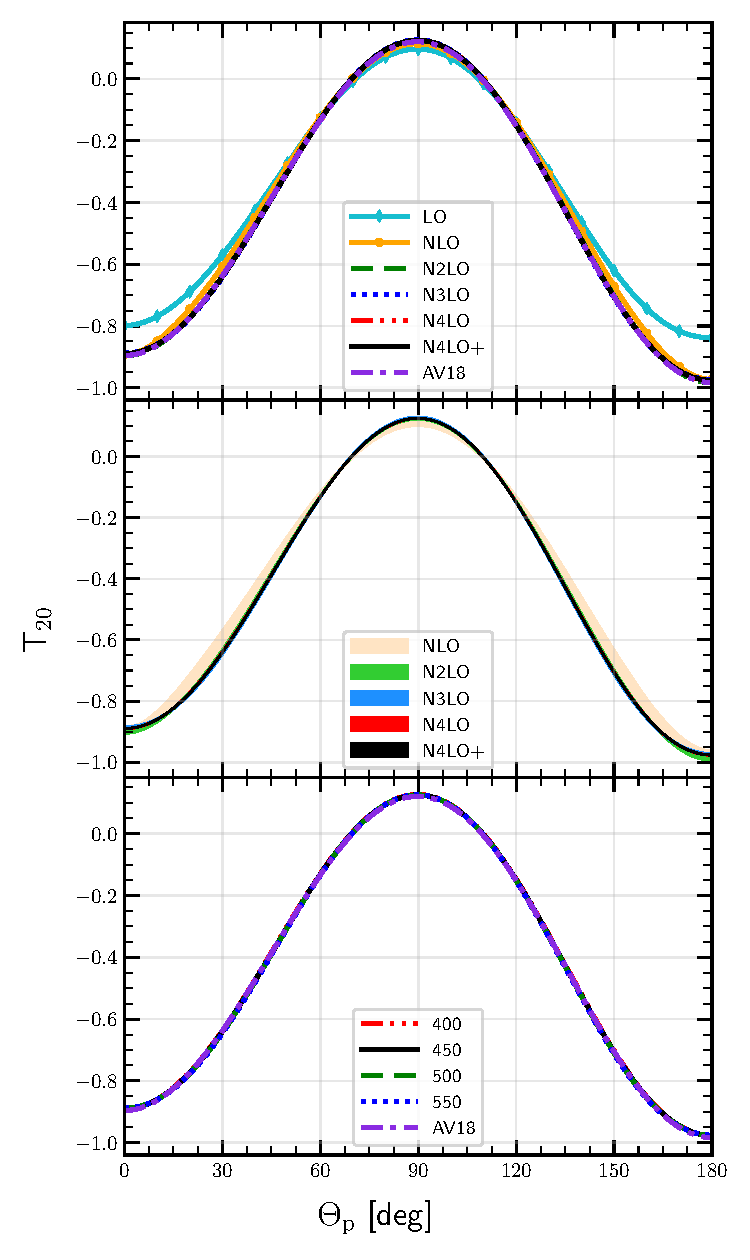
\includegraphics[width=\textwidth]{Figures_De/T20D2_30mev.pdf}
            \caption{T$_{20}$}
            \label{T20_30_vert}
        \end{subfigure}
        \begin{subfigure}[b]{0.46\textwidth}
            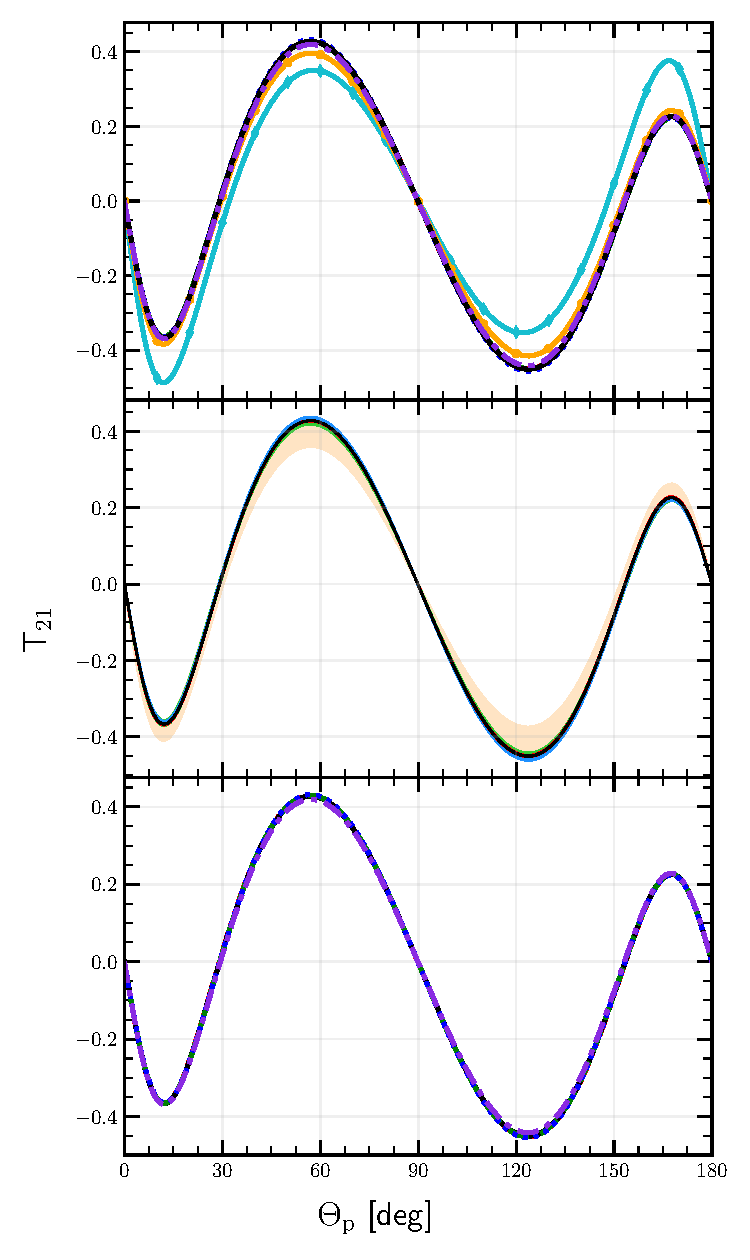
\includegraphics[width=\textwidth]{Figures_De/T21D2_30mev.pdf}
            \caption{T$_{21}$}
            \label{T21_30_vert}
        \end{subfigure}
        \caption{Tensor analyzing power T$_{20}$  {\bf (a)}
        and T$_{21}$ {\bf (b)}
        as a function of the outgoing proton angle in the center of mass frame 
        for the photon's energy \SI{30}{\mev}.
        Top row presents results obtained using potential
        with different chiral orders (from LO to N$^4$LO+) with cutoff parameter $\Lambda=\SI{450}{\mev}$.
        The middle row shows truncation errors for each 
        chiral order starting from NLO and
        bottom row presents a cutoff dependency (chiral potential N$^4$LO+).
        For the sake of comparison, predictions obtained with \gls*{av18} potential are on figures as well.}
        \label{T20_T21_30}
    \end{figure}

    \begin{figure}[htb]
        \centering
        \begin{subfigure}[b]{0.46\textwidth}
            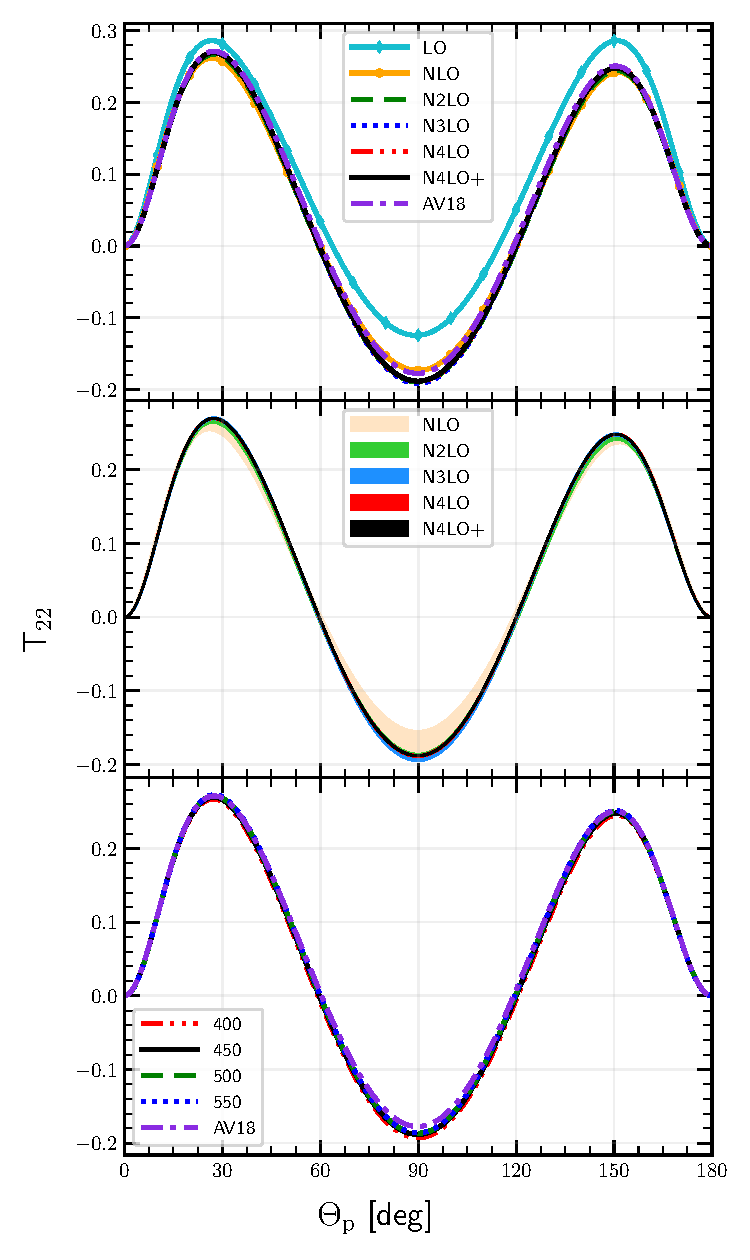
\includegraphics[width=\textwidth]{Figures_De/T22D2_30mev.pdf}
            \caption{T$_{22}$}
            \label{T22_30_vert}
        \end{subfigure}
        \begin{subfigure}[b]{0.46\textwidth}
            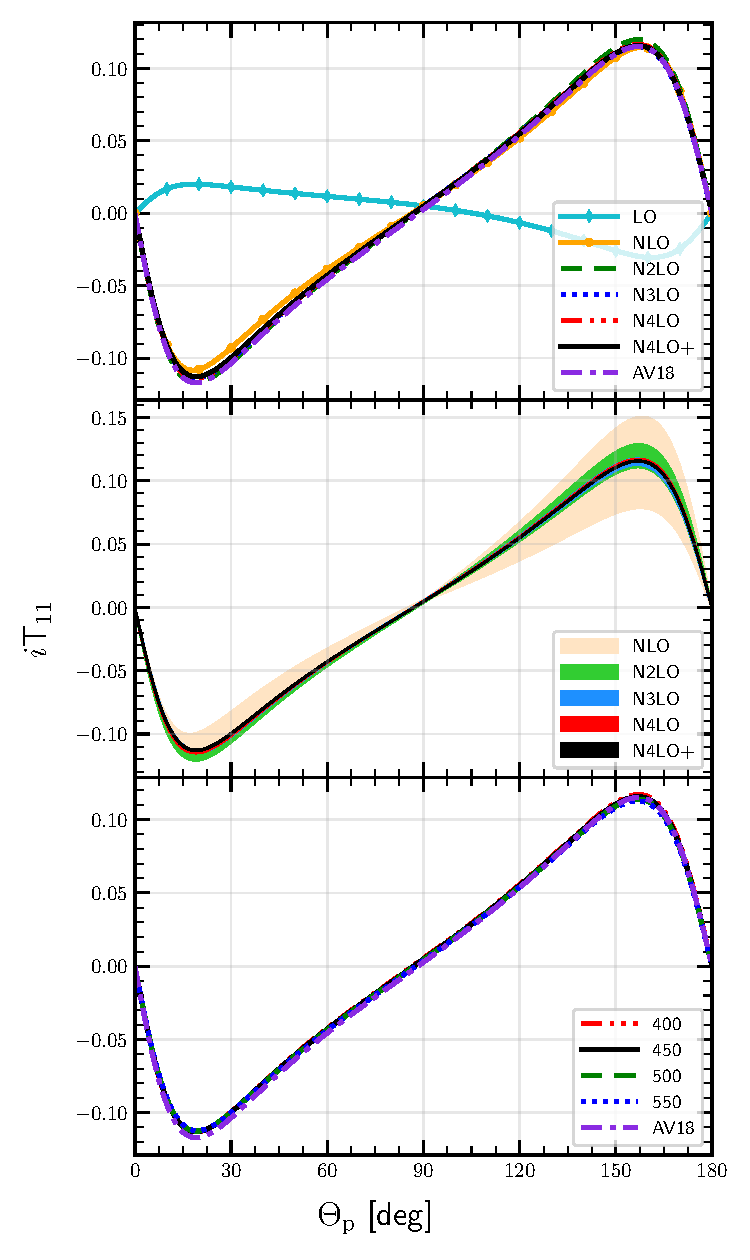
\includegraphics[width=\textwidth]{Figures_De/T11D2_30mev.pdf}
            \caption{iT$_{11}$}
            \label{T11_30_vert}
        \end{subfigure}
        \caption{The same as on \ref{T20_T21_30} but for polarisation observables
        T$_{22}$ (subfigure {\bf (a)}) and iT$_{11}$ (subfigure {\bf (b)}).}
        \label{T22_T11_30}
    \end{figure}

    \begin{figure}[htb]
        \centering
        \begin{subfigure}[b]{0.46\textwidth}
            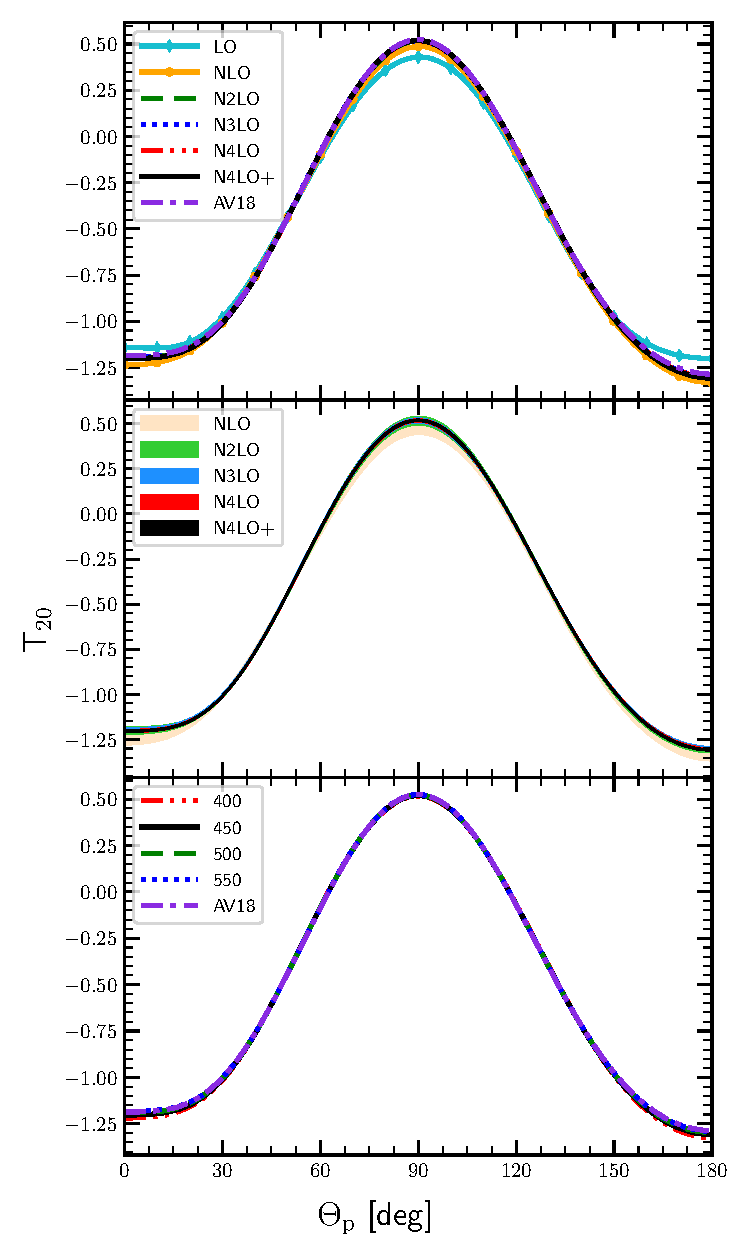
\includegraphics[width=\textwidth]{Figures_De/T20D2_100mev.pdf}
            \caption{T$_{20}$}
            \label{T20_100_vert}
        \end{subfigure}
        \begin{subfigure}[b]{0.46\textwidth}
            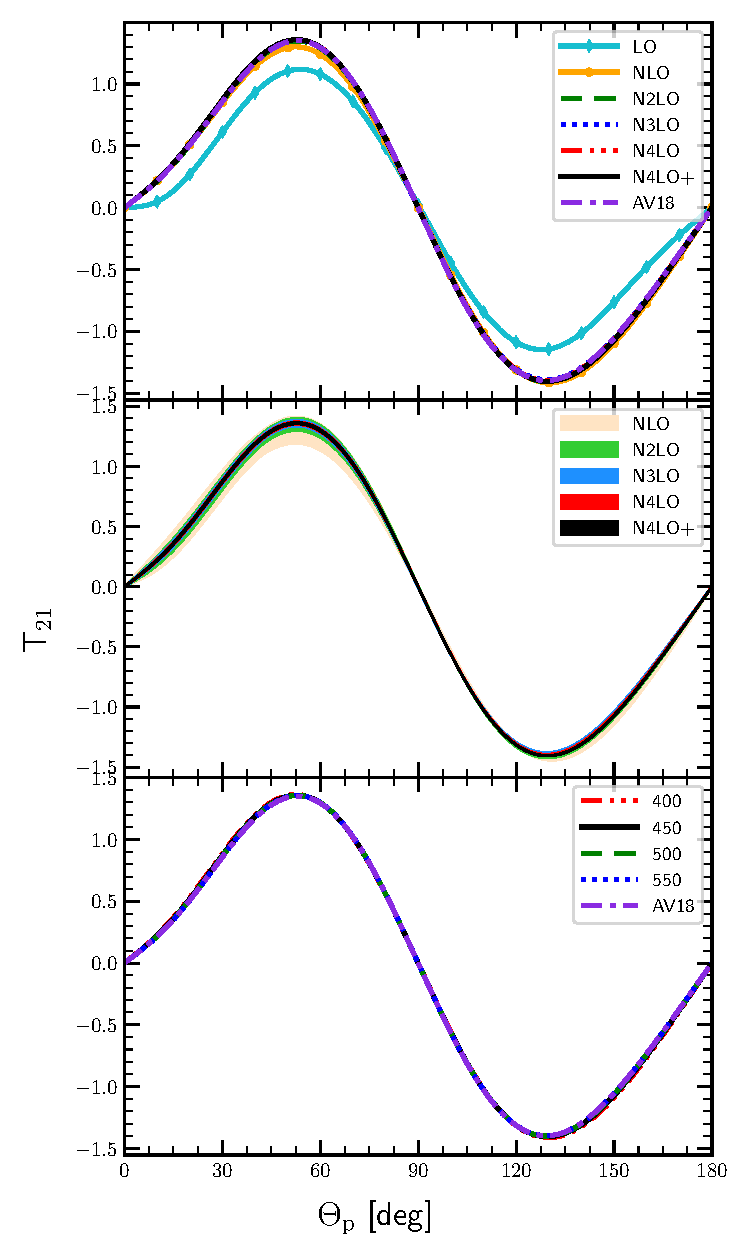
\includegraphics[width=\textwidth]{Figures_De/T21D2_100mev.pdf}
            \caption{T$_{21}$}
            \label{T21_100_vert}
        \end{subfigure}
        \caption{Tensor analyzing power T$_{20}$  {\bf (a)}
        and T$_{21}$ {\bf (b)}
        as a function of the outgoing proton angle in the center of mass frame 
        for the photon's energy \SI{100}{\mev}.
        Top row presents results obtained using potential
        with different chiral orders (from LO to N$^4$LO+) with cutoff parameter $\Lambda=\SI{450}{\mev}$.
        The middle row shows truncation errors for each 
        chiral order starting from NLO and
        bottom row presents a cutoff dependency (chiral potential N$^4$LO+).
        For the sake of comparison, predictions obtained with \gls*{av18} potential are on figures as well.}
        \label{T20_T21_100}
    \end{figure}

    \begin{figure}[htb]
        \centering
        \begin{subfigure}[b]{0.46\textwidth}
            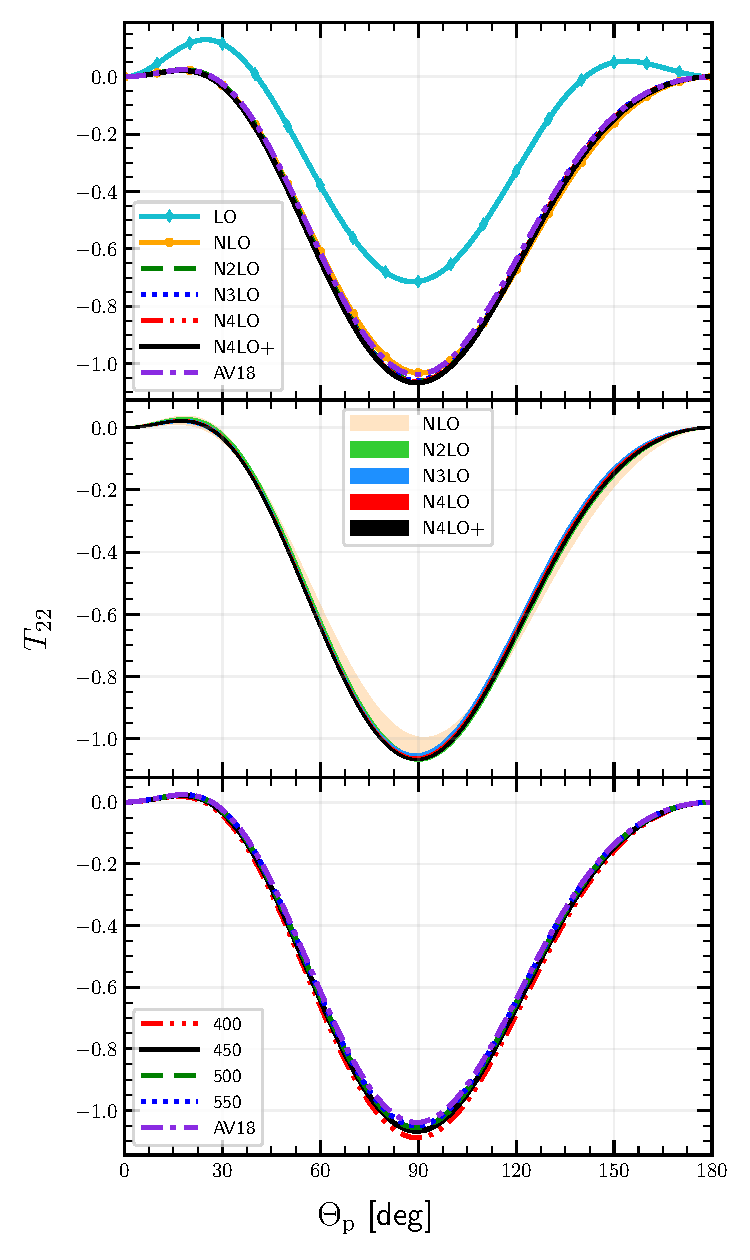
\includegraphics[width=\textwidth]{Figures_De/T22D2_100mev.pdf}
            \caption{T$_{22}$}
            \label{T22_100_vert}
        \end{subfigure}
        \begin{subfigure}[b]{0.46\textwidth}
            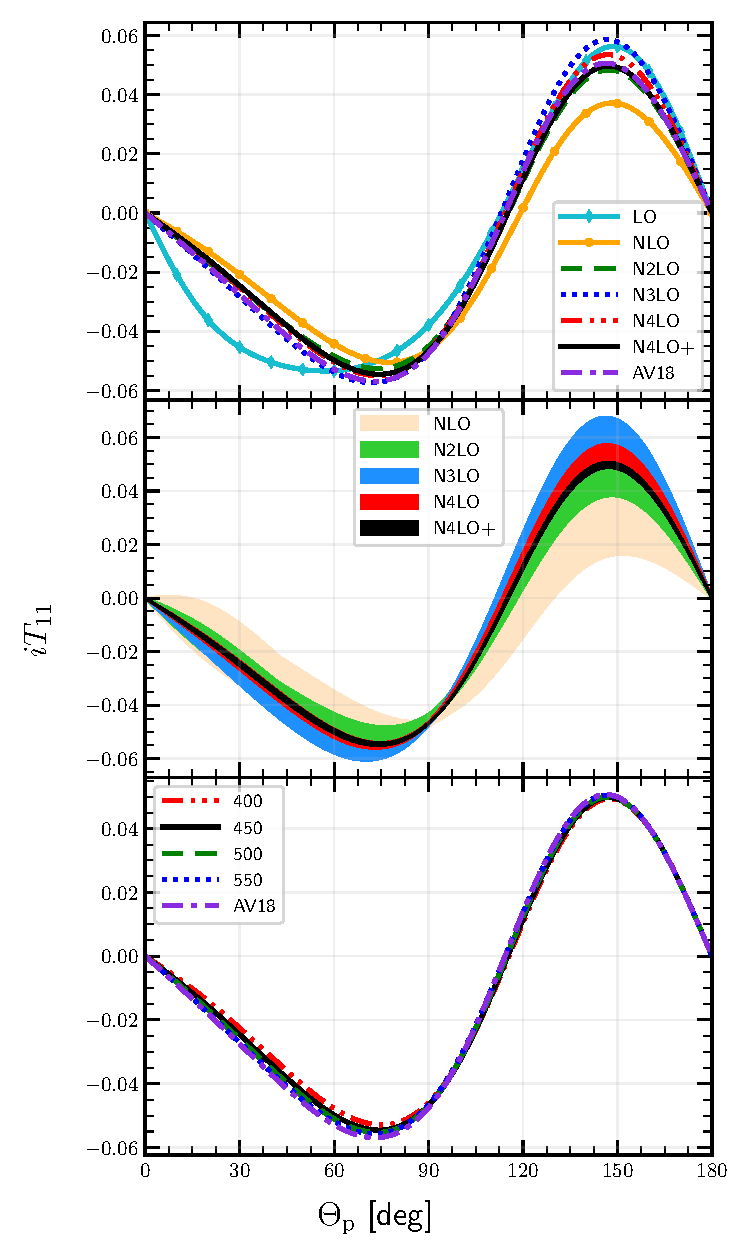
\includegraphics[width=\textwidth]{Figures_De/T11D2_100mev.pdf}
            \caption{iT$_{11}$}
            \label{T11_100_vert}
        \end{subfigure}
        \caption{The same as on \ref{T20_T21_100} but for polarisation observables
        T$_{22}$ (subfigure {\bf (a)}) and iT$_{11}$ (subfigure {\bf (b)}).}
        \label{T22_T11_100}
    \end{figure}

    In \fig{tensor_pw_1nc} together with best prediction at $\text{E}_\gamma = \SI{30}{\mev}$ (N$^4$LO+, $\Lambda=\SI{450}{\mev}$, Siegert theorem),
    I show predictions obtained with 1NC only and with plane-wave contribution without rescattering part.
    In case of deuteron's tensor analyzing power components, the contribution of rescattering part is not that 
    big for T$_{20}$, T$_{21}$ and T$_{22}$ (up to \SI{20}{\percent} in extremum points). Nevertheless, for
    $i$T$_{11}$ we see that PW part equals to zero. It may be connected with some features of this particular
    components, such that plane-wave part cancels out.
    The 2NC component taken into account via Siegert theorem has a dominant contribution here. We see that 
    1NC predictions are absolutely away from the Full predictions and in case of $i$T$_{11}$
    does not even reflect total prediction qualitatively.

    \begin{figure}[h]
        \begin{center}
        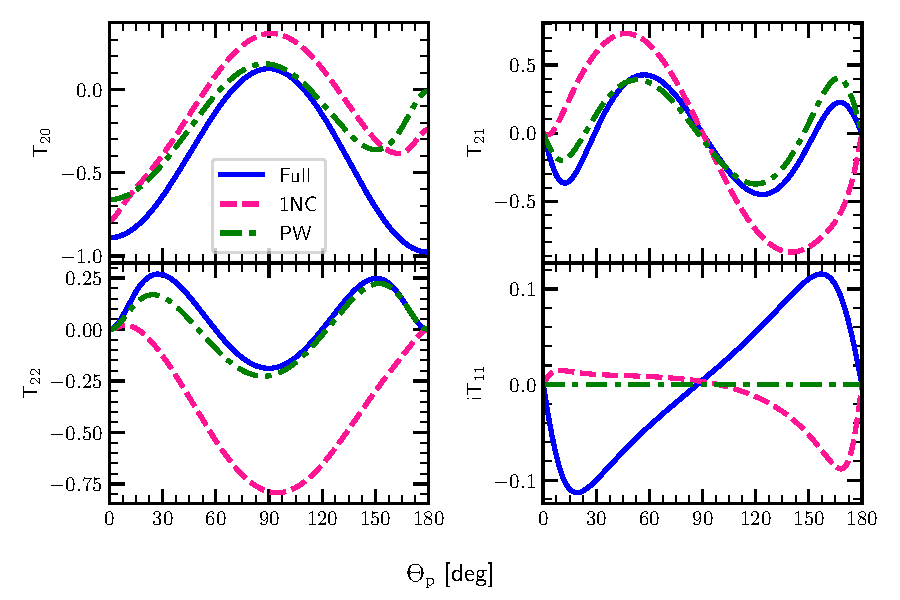
\includegraphics[width=0.9\textwidth]{Figures_De/TensorPowers_pw_1nc.pdf}
        \end{center}
        \caption{Tensor analyzing power components T$_{20}$, T$_{21}$, T$_{22}$ and $i$T$_{11}$ as a functions of the
        outgoing proton angle $\theta_p$ (in the center of mass frame) at $\text{E}_\gamma = \SI{30}{\mev}$. Similarly to \fig{Diff_cross_pw_1nc} predictions obtained with chiral N$^4$LO+ potential and $\Lambda=\SI{450}{\mev}$ are presented for each component.
        Blue solid line is a best predictions we have (plane-wave plus rescattering parts, 1NC + Siegert), pink dashed line shows predictions obtained with
        single-nucleon current only (without Siegert contributions) and green dashed-dotted line
        is a prediction with plane-wave part only - without rescattering.}
        \label{tensor_pw_1nc}
    \end{figure}

    \fig{tensor_pw_1nc_100mev} presents similar results but for E$_\gamma = \SI{30}{\mev}$
    and it is intersting that difference between Full and 1NC prediction becomes smaller
    and it is especially visible for $T_{22}$. At this energy the relative difference 
    at $\theta_p = \ang{90}$ is \SI{43.6}{\percent} comparing to \SI{122.8}{\percent}
    at E$_\gamma = \SI{30}{\mev}$. Similarly, the difference for T$_{20}$
    at E$_\gamma = \SI{30}{\mev}$($\theta_p = \ang{90}$) is \SI{91.4}{\percent}
    and at E$_\gamma = \SI{100}{\mev}$ it drops down to \SI{28.8}{\percent}.
    This trend is noticeable looking on Figures (\ref{tensor_angular_25-45} - \ref{tensor_angular_230-330}). With 

    \begin{figure}[h]
        \begin{center}
        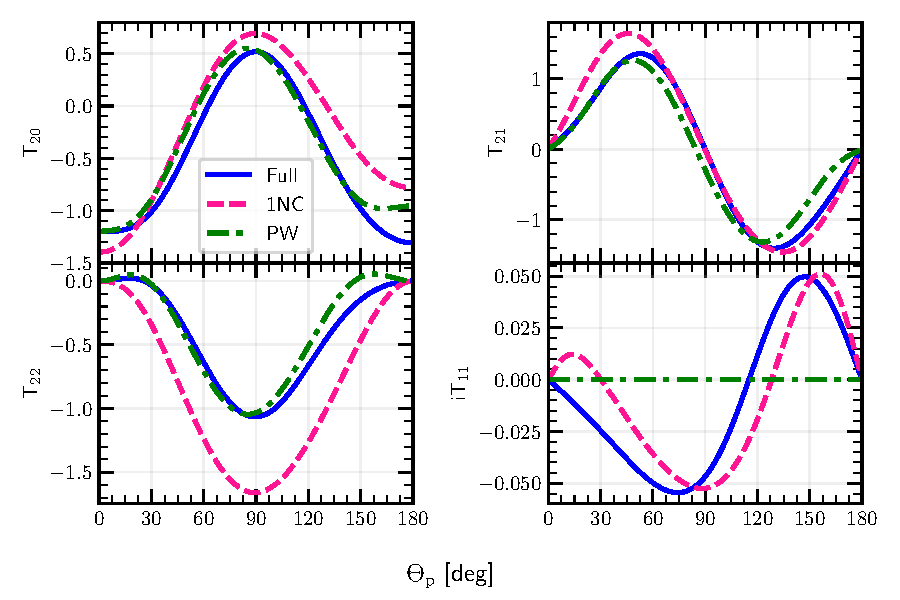
\includegraphics[width=0.9\textwidth]{Figures_De/TensorPowers_100mev_pw_1nc.pdf}
        \end{center}
        \caption{The same as on \fig{tensor_pw_1nc} but for E$_\gamma=\SI{100}{\mev}$}
        \label{tensor_pw_1nc_100mev}
    \end{figure}


    
    On the next figures, I show the predictions in a similar way as it was done
    in \cite{rachek2007} in order to compare my predictions with the experimental
    data. On the Figures \ref{tensor_angular_25-45} - \ref{tensor_angular_230-330}
    I show an angular dependance of the $T_{2i}$ ($i=0,1,2$) for a specific energy bands.
    Solid blue line shows an average value of the observable in the specified energy range
    obtained at N$^4$LO+ with $\Lambda=\SI{450}{\mev}$, while the pink dashed line is a prediction
    obtained with a same setup but without using a contributions from Siegert approach
    (single nucleon current only). Bands for each of prediction specify the spread of
    predictions in regarded energy band.
    
    One can see that the data description is better for the predictions with Siegert contributions 
    and SN current is not able to describe experiment properly. With increasing energy 
    (more than \SI{100}{\mev}),
    the difference between predicted values and experimental data becomes larger
    (especially for $T_{22}$), but the model I use is not meant to be used for high energies 
    and figures are presented out of the curiosity. 
    




    \begin{figure}[h]
        \begin{center}
        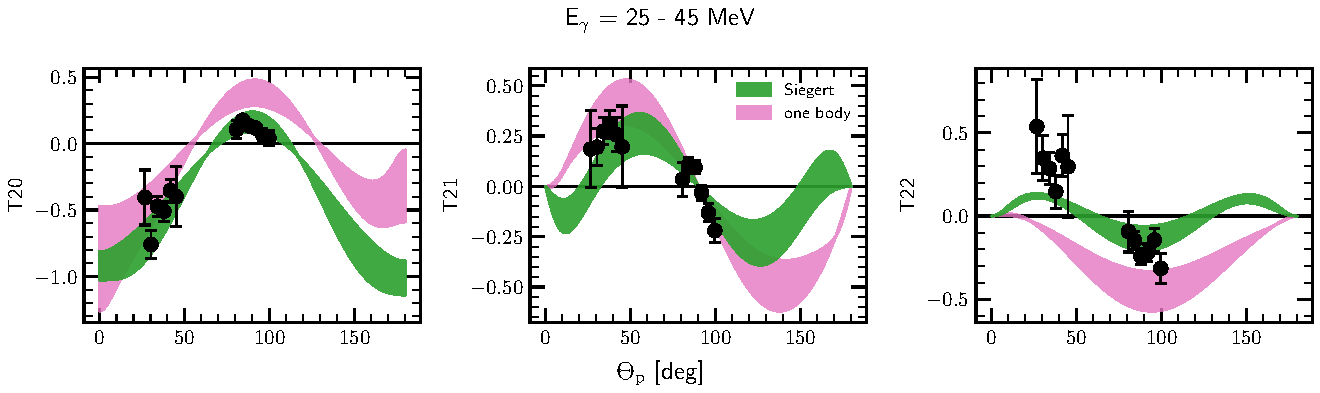
\includegraphics[width=1\textwidth]{Figures_De/Tensor_analyzing_power_angular_E25-45.pdf}
        \end{center}
        \caption{Tensor analyzing powers T$_{20}$, T$_{21}$ and T$_{22}$ as a functions of the
        outgoing proton angle $\theta_p$ (in the center of mass frame).
        Solid blue line is a mean value of my predictions obtained with a
        \gls*{sms} potential at N$^4$LO+ chiral order and with $\Lambda$~=~450~MeV
        at energy values from \SIrange[range-phrase=\text{ to }]{25}{45}{\mev} and
        where SN current was used together with Siegert approach. 
        Pink dashed line is similar prediction but with SN only. 
        The corresponding bands show the deviation of predictions in the regarded
        energy region.
        % Filled bands show maximal spread of my predictions obtained with a 
        % \gls*{sms} potential at N$^4$LO+ chiral order and with $\Lambda$~=~450~MeV
        % for the energy span from 25 to 45 MeV. Blue bands correspond to the
        % case where SN current was used together with Siegert approach and 
        % pink bands - to the SN currentonly. 
        Filled circles are experimental data
        from \cite{rachek2007} for the analogous energy span.}
        \label{tensor_angular_25-45}
    \end{figure}

    \begin{figure}[h]
        \begin{center}
        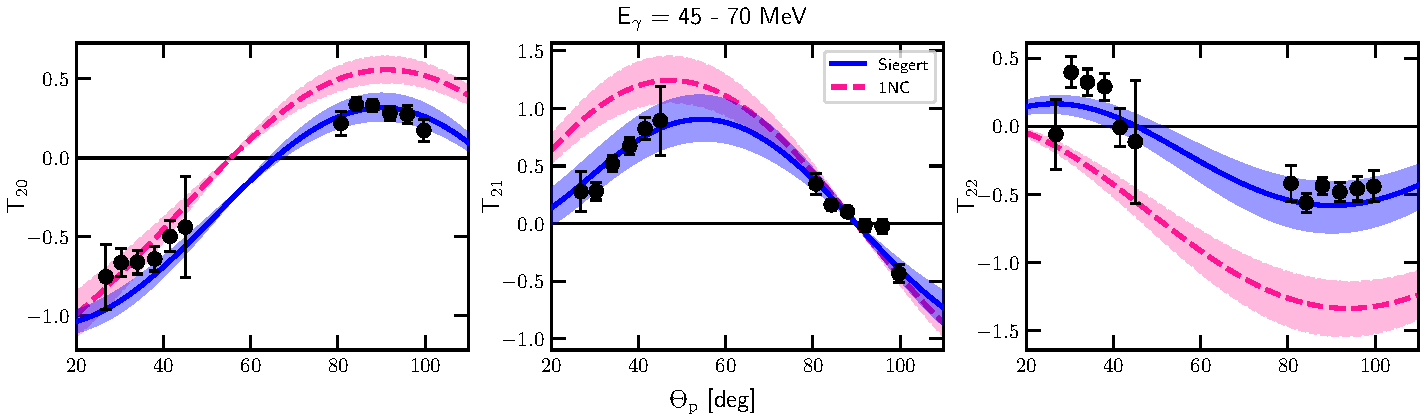
\includegraphics[width=0.95\textwidth]{Figures_De/Tensor_analyzing_power_angular_E45-70.pdf}
        \end{center}
        \caption{The same as on the Fig.~\ref*{tensor_angular_25-45} but for energy bin \SIrange{45}{70}{\mev}}
        \label{tensor_angular_45-70}
    \end{figure}

    \begin{figure}[h]
        \begin{center}
        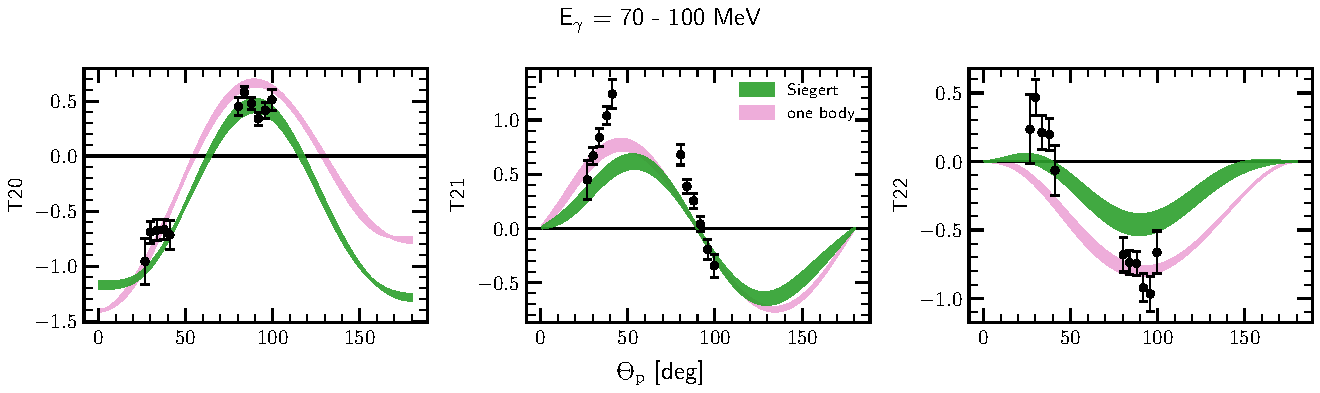
\includegraphics[width=0.95\textwidth]{Figures_De/Tensor_analyzing_power_angular_E70-100.pdf}
        \end{center}
        \caption{The same as on the Fig.~\ref*{tensor_angular_25-45} but for energy bin \SIrange{70}{100}{\mev}}
        \label{tensor_angular_70-100}
    \end{figure}        

    \begin{figure}[h]
        \begin{center}
        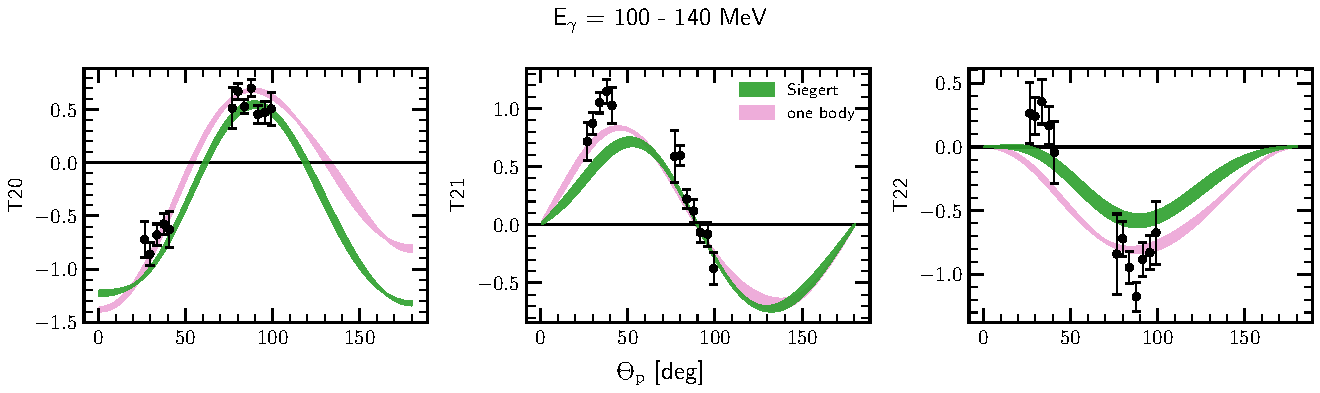
\includegraphics[width=0.95\textwidth]{Figures_De/Tensor_analyzing_power_angular_E100-140.pdf}
        \end{center}
        \caption{The same as on the Fig.~\ref*{tensor_angular_25-45} but for energy bin \SIrange{100}{140}{\mev}}
        \label{tensor_angular_100-140}
    \end{figure}
        
        

    \begin{figure}[h]
        \begin{center}
        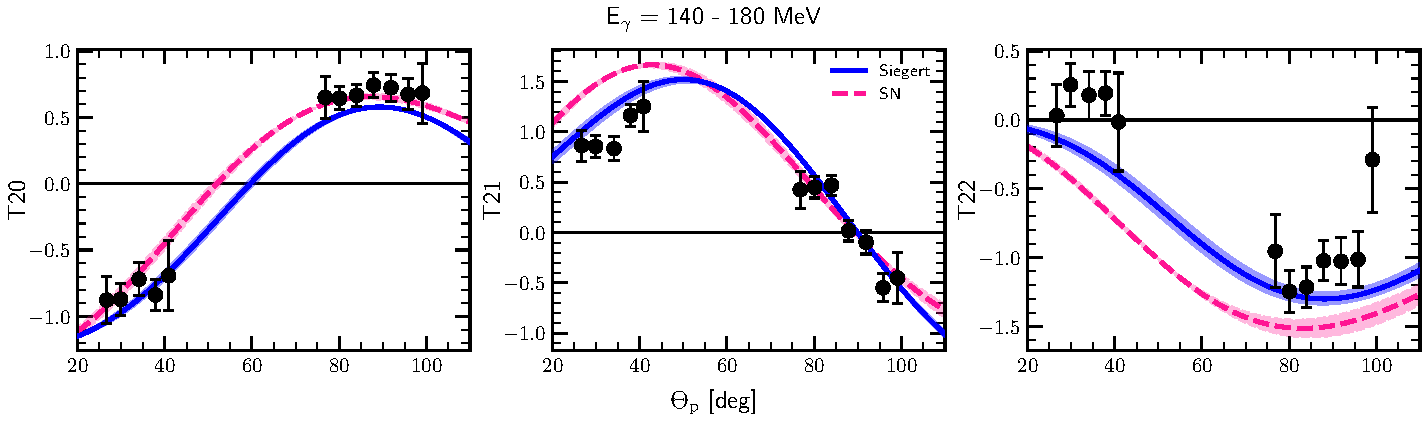
\includegraphics[width=0.95\textwidth]{Figures_De/Tensor_analyzing_power_angular_E140-180.pdf}
        \end{center}
        \caption{The same as on the Fig.~\ref*{tensor_angular_25-45} but for energy bin \SIrange{140}{180}{\mev}}
        \label{tensor_angular_140-180}
    \end{figure}
        

    \begin{figure}[h]
        \begin{center}
        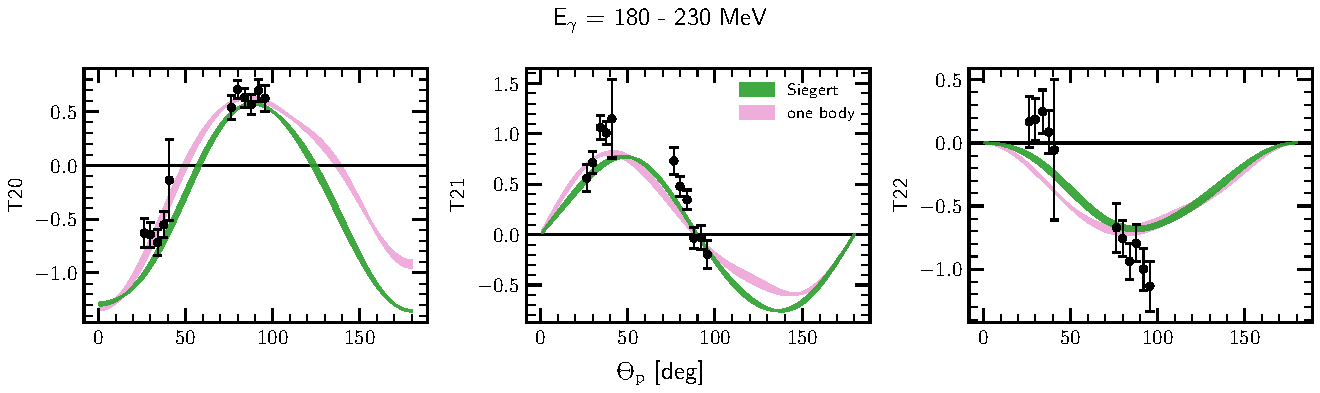
\includegraphics[width=0.95\textwidth]{Figures_De/Tensor_analyzing_power_angular_E180-230.pdf}
        \end{center}
        \caption{The same as on the Fig.~\ref*{tensor_angular_25-45} but for energy bin \SIrange{180}{230}{\mev}}
        \label{tensor_angular_180-230}
    \end{figure}

    \begin{figure}[h]
        \begin{center}
        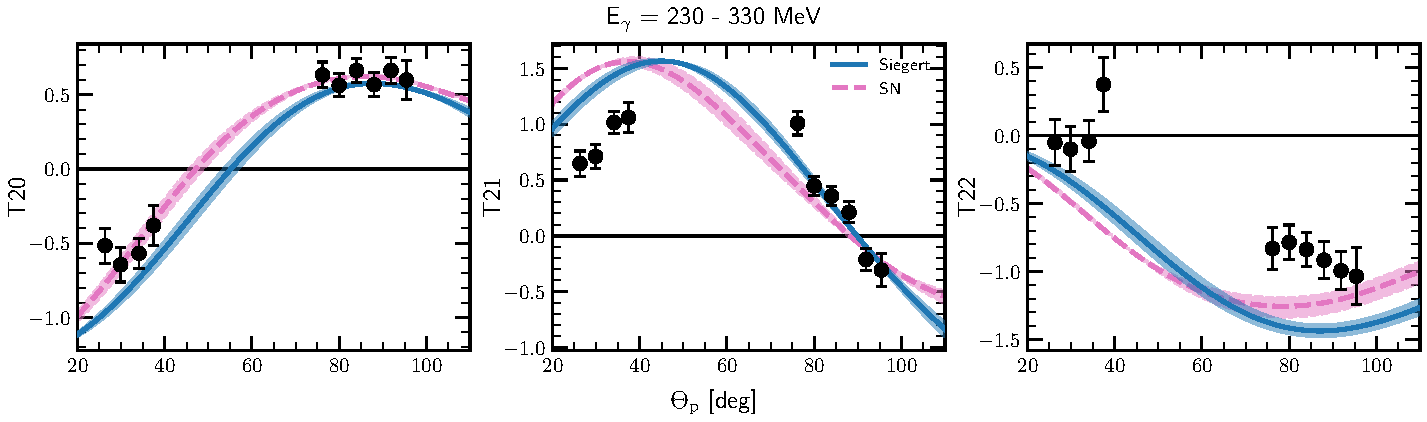
\includegraphics[width=0.95\textwidth]{Figures_De/Tensor_analyzing_power_angular_E230-330.pdf}
        \end{center}
        \caption{The same as on the Fig.~\ref*{tensor_angular_25-45} but for energy bin \SIrange{230}{330}{\mev}}
        \label{tensor_angular_230-330}
    \end{figure}
        


    On the Figure \ref{T20_vs_en} the energy dependance of $T_{20}$ and $T_{22}$
    (integrated over all angles)
    is presented for the energy range 0-400~MeV. I also demonstrate the experimental data from
    \cite{rachek2007} and \cite{mishev1993} as well as theoretical calculations from \cite{Schmitt1989}
    on the figure. For $T_{20}$ the model is able to describe experimental data well even for
    high energies. On the other hand, $T_{22}$ is not so well described: for the low 
    energies the prediction curve is somehow within uncertainties of experimental data,
    but further the difference with the data becomes larger. Also it is not 
    reflect the qualitative nature of the data as we can see that after around 150~MeV
    data points start ascending which is not represented in my predictions.
    Theoretical predictions from \cite{Schmitt1989} (brown dashed curve) are also not able
    to describe data quantitatively for $T_{22}$, but the growth is presented there. 

    Similar situation is on the Figures \ref{tensor_energy_24-48} and \ref{tensor_energy_70-102}
    where I show an energy dependance of deuteron analyzing power components for 
    specific angular ranges (following the data from \cite{rachek2007}).
    Predictions for $T_{20}$ are able to reflect the experimental results,
    while for $T_{21}$ and $T_{22}$ predictions are reasonable (quantitative-wise) 
    only for lower energies and difference with data becomes larger
    when energy increases. Predictions for $T_{22}$ once more 
    confirm an insufficiency of SN and an importance of
    2-nucleon current contributions. 
    

    \begin{figure}[h]
        \begin{center}
        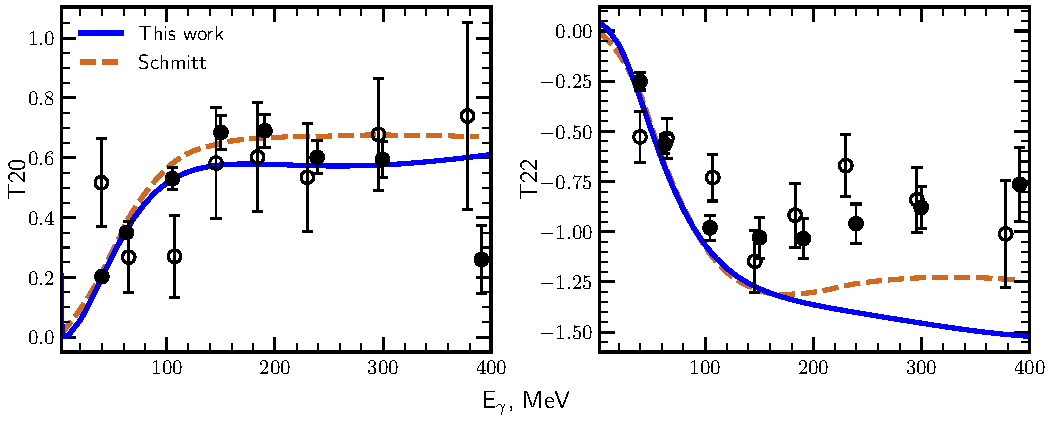
\includegraphics[width=0.9\textwidth]{Figures_De/T20_T22_vs_en.pdf}
        \end{center}
        \caption{Tensor analyzing powers T$_{20}$ and T$_{22}$ as a functions of the photon energy E$_\gamma$
        with fixed outgoing proton angle $\theta_p = 88^{\circ}$ (in the center of mass frame).
        My predictions (blue solid line) are obtained with \gls*{sms} potential at chiral order N$^4$LO+
        and with cutoff parameter $\Lambda = \SI{450}{\mev}$ with 2NC contributions included via Siegert theorem,
        dashed pink line show prediction obtained without 2NC contributions.
        Dashed-dotted brown line presents calculations from \cite{Schmitt1989}.
        Experimental data is taken from \cite{rachek2007} (filled circles)
        and \cite{mishev1993} (empty circles).}
        \label{T20_vs_en}
    \end{figure}

    \begin{figure}[h]
        \begin{center}
        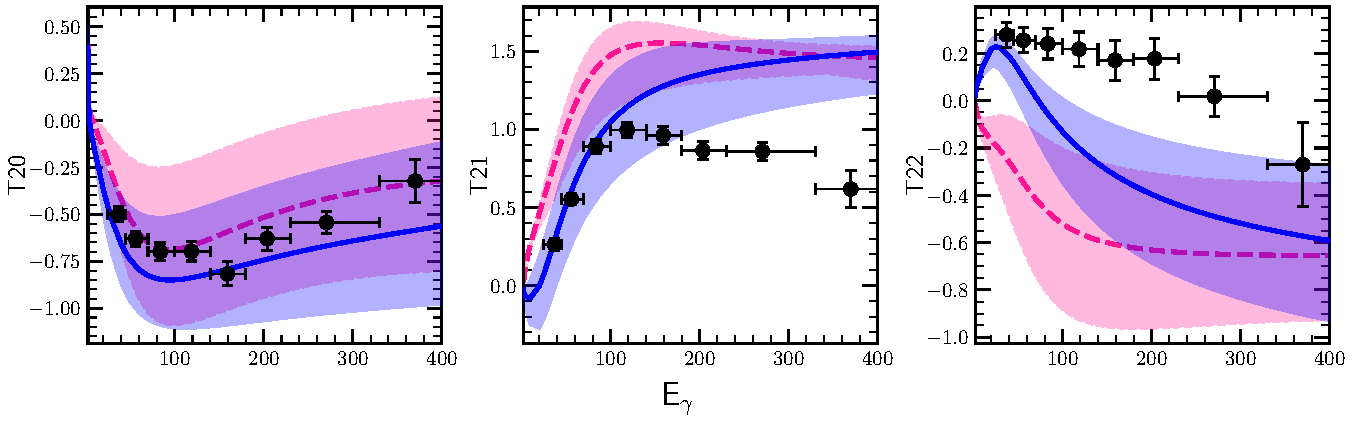
\includegraphics[width=0.95\textwidth]{Figures_De/TensorPower_Th24-48.pdf}
        \end{center}
        \caption{Tensor analyzing powers T$_{20}$, T$_{21}$ and T$_{22}$ as a functions of the
        photon's energy within the outgoing proton's angle range $24^{\circ} - 48^{\circ}$
        (in the center of mass frame).
        Solid blue line is a mean value of my predictions obtained with
        \gls*{sms} potential at N$^4$LO+ chiral order and with $\Lambda$~=~450~MeV
        at energy values from 25 to 45 MeV within
        a given angles range and
        where SN current was used together with Siegert approach. 
        Pink dashed line is similar prediction but with SN only. 
        The corresponding bands show the deviation of predictions in the regarded
        energy region.
        Filled circles are experimental data
        from \cite{rachek2007} for the analogous energy span.}
        \label{tensor_energy_24-48}
    \end{figure}

    \begin{figure}[h]
        \begin{center}
        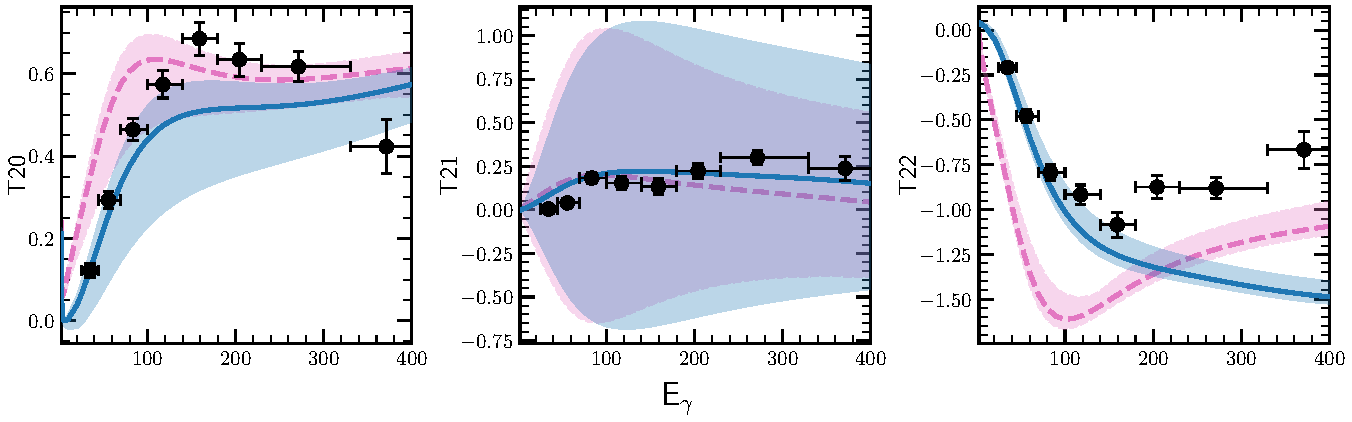
\includegraphics[width=0.95\textwidth]{Figures_De/TensorPower_Th70-102.pdf}
        \end{center}
        \caption{The same as on the Fig.~\ref*{tensor_energy_24-48} but
        for the angles' range $70^{\circ} - 102^{\circ}$.}
        \label{tensor_energy_70-102}
    \end{figure}
    
    On the \fig{assymetry} I demonstrate predictions
    for the photon asymmetry $\Sigma_\gamma$ for the 
    deuteron photodisintegraion with $E_\gamma$~=~20~MeV (a)
    and 60~MeV(b) as well as experimental data.
    Both (a) and (b) figureas are organized similarly to the 
    figures I showed earlier for the tensor analyzing power (e.g. \fig{T22_T11_30}).
    That is the top pane is aimed to demonstrate predictions obtained
    with chiral potential at different orders, the middle 
    one is showing a truncation error bands and the bottom - shows 
    the cutoff dependance. What we can see here is good 
    convergence with respect to the chiral order. For both regarded 
    energies predictions at different orders are very close to each other
    except for LO and NLO curves. Nevertheless, at 60~MeV we can see 
    that truncation error bands reveal some uncertainty connected 
    with the chiral order and I can assume that even some higher chiral 
    orders would still contribute to the predictions at this energy.

    Cutoff dependance is also stronger at 60~MeV. We can clearly see
    that predictions are different for each value of the $\Lambda$.
    The standard deviation with respect to the cutoff parameter at 20~MeV
    does not exceed 0.7\% of the mean value while at the photon's energy 60~MeV
     the maximum value is around 2.5\% (at $\theta = 115^\circ$).

     Regarding the correspondace to experimental data, we can clearly see that
     for the lower energy predictions are almost perfectly overlaping
     with exparimental point (and error bars). Few points are laying
     outside the predictions but it can be caused by experimental issues.
     For 60~MeV, experimental data points are constantly below prediction
     curves (especially in the middle of angles range). It seems that some systematic 
     uncertainty is presented in predictions and multiplication by some factor
     (presumably less than 1)
     could help predictions be more similar to experimental data.

     On the \fig{asymmetry_90deg} I present dependance of the asymmetry
     $\Sigma_\gamma$ on the photon's energy with fixed value
     of the outgoing proton's angle $\theta_p = 90^\circ$ 
     (following the data given at \cite{delbianco_1981} and \cite{depascale_asymmetry}).
     It is noticeable that with increasing energy, the prediction curve
     becomes more and more above the experimental data. This trend
     was also observed in angular dependance of the asymmetry at 60~MeV
     so I can assume that within our framework, 
     $\Sigma_\gamma$ is sensitive to the initial photon's energy and some 
     contributions are missing in order to prepare good predictions
     at higher energies. From the \fig{asymmetry_90deg} we can say that
     large descripancy with data starts appearing after 
     35~MeV. 

    \begin{figure}[h]
        \centering
        \begin{subfigure}[b]{0.46\textwidth}
            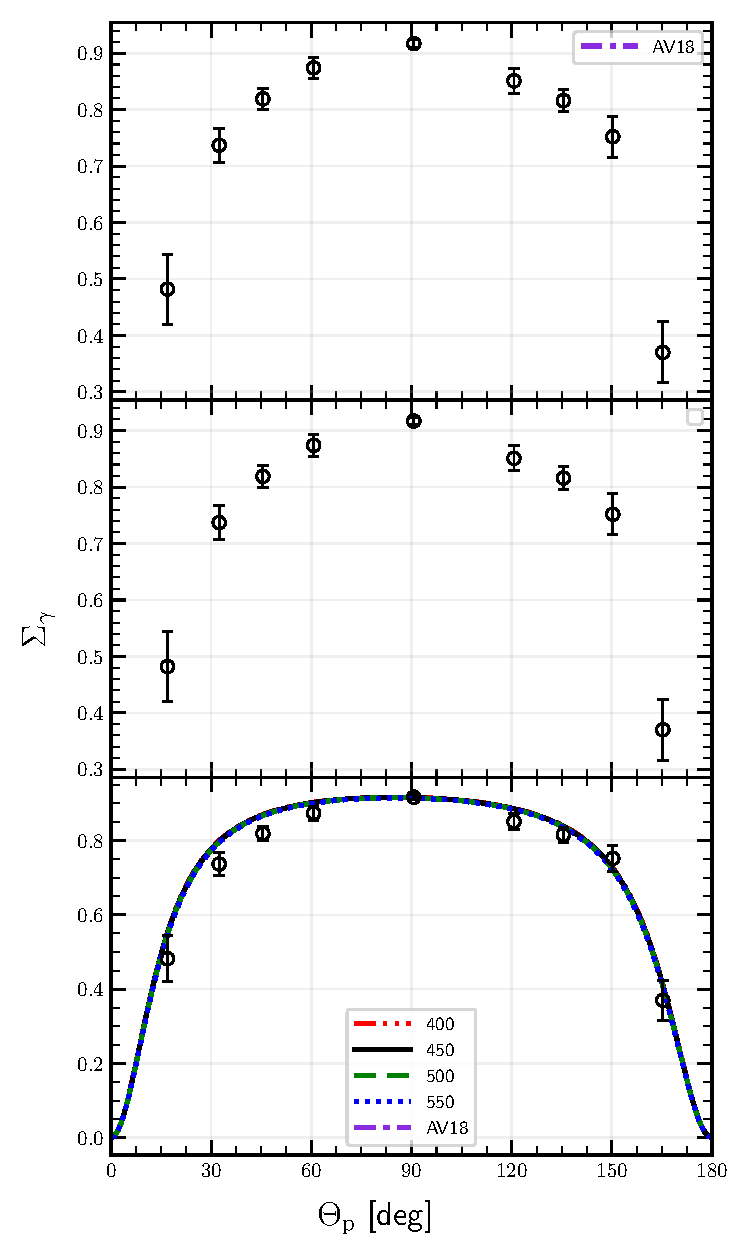
\includegraphics[width=\textwidth]{Figures_De/AX2_20mev.pdf}
            \caption{\small E$_\gamma = \SI{20}{\mev}$}
            \label{AX_20_vert}
        \end{subfigure}
        \begin{subfigure}[b]{0.46\textwidth}
            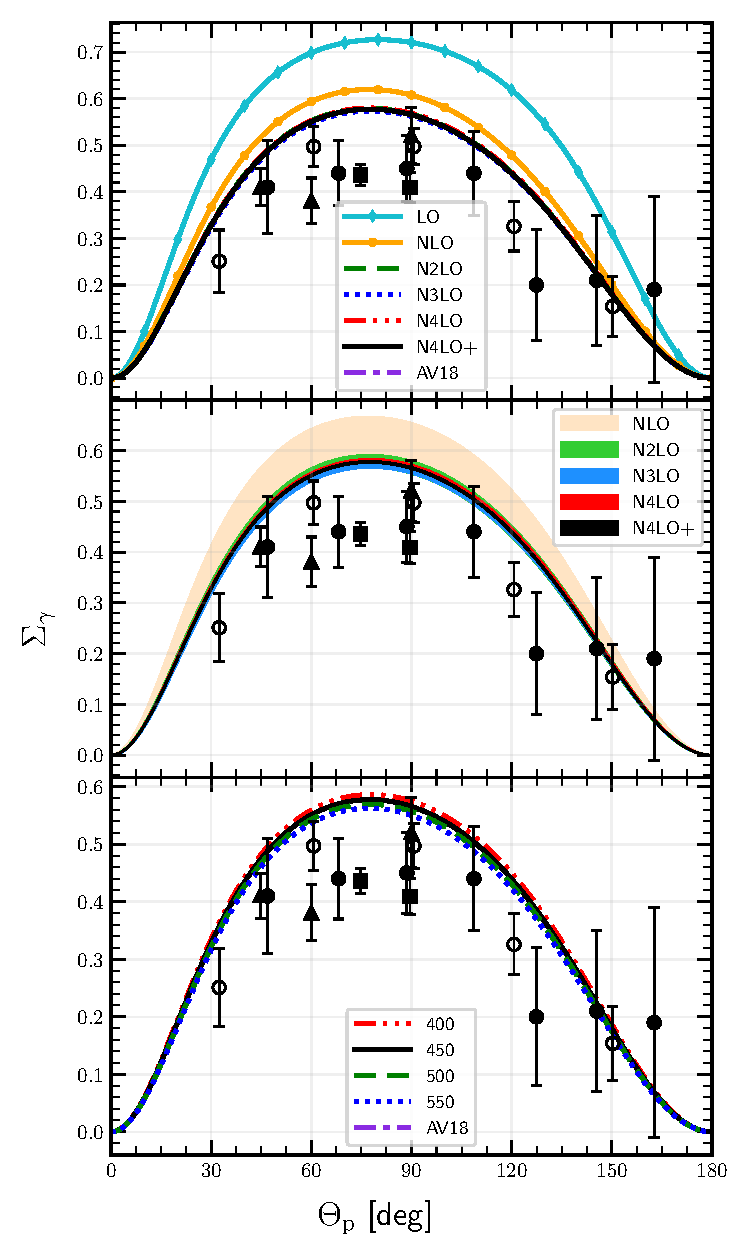
\includegraphics[width=\textwidth]{Figures_De/AX2_60mev.pdf}
            \caption{\small E$_\gamma = \SI{60}{\mev}$}
            \label{AX_60_vert}
        \end{subfigure}
        \caption{The photon asymmetry $\Sigma_\gamma$ 
        as a function of the outgoing proton angle in the center of mass frame 
        for the photon's energy \SI{30}{\mev}(a) and \SI{100}{\mev}(b).
        Top row presents results obtained using potential
        with different chiral orders (from LO to N$^4$LO+) with cutoff parameter $\Lambda=\SI{450}{\mev}$.
        The middle row shows truncation errors for each 
        chiral order starting from NLO and
        bottom presents a cutoff dependency (chiral potential N$^4$LO+).
        Filled circles are experimental data from \cite{KRAUSE1992_asymetry},
        empty circles - from \cite{depascale_asymmetry}, filled squares
        - from \cite{Barannik_asymetry} and triangles are from \cite{Vnukov_asymmetry}.
        For the sake of comparison, predictions obtained with \gls*{av18} potential are on  figures as well.}
        \label{assymetry}
    \end{figure}
     
    \begin{figure}[h]
        \begin{center}
        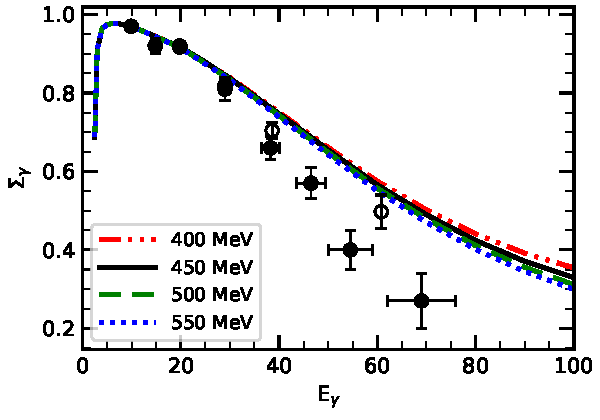
\includegraphics[width=0.75\textwidth]{Figures_De/AX2_90deg.pdf}
        \end{center}
        \caption{The photon asymmetry $\Sigma_\gamma$ 
        as a function of the photon energy  
        with fixed outgoing proton angle $\theta_p=90^\circ$.
        Each curve corresponds to the particular value of the cutoff parameter
        and chiral potential used here is N$^4$LO+.
        Filled circles are experimental data from \cite{delbianco_1981},
        empty circles - from \cite{depascale_asymmetry}.}
        \label{asymmetry_90deg}
    \end{figure}
    

    The proton polarization is demonstrated on the \fig{PY_30_100_vert} for the 
    photon's energy 30~MeV(a) and 100~MeV(b). In this case even higher energy
    such as 100~MeV does not reveal neither
    slower convergence with respect to the chiral order no
    stronger cutoff dependence. Figures for both energies show
    that only next-to-leading order brings relatively high contribution
    while taking into account each subsequent order does not change predictions
    largely. In the case of cutoff dependance, we see that curves for each
    value of $\Lambda$ are very close to each other. 
    The standard deviation of the predictions with respect to the cutoff parameter
    has maximal value 1.94\% at $E_\gamma = 30$MeV and 3.2\% at 100~MeV.
    The dependance is slightly stronger for higher energy, but these values are comparable.


    \begin{figure}[h]
        \centering
        \begin{subfigure}[b]{0.46\textwidth}
            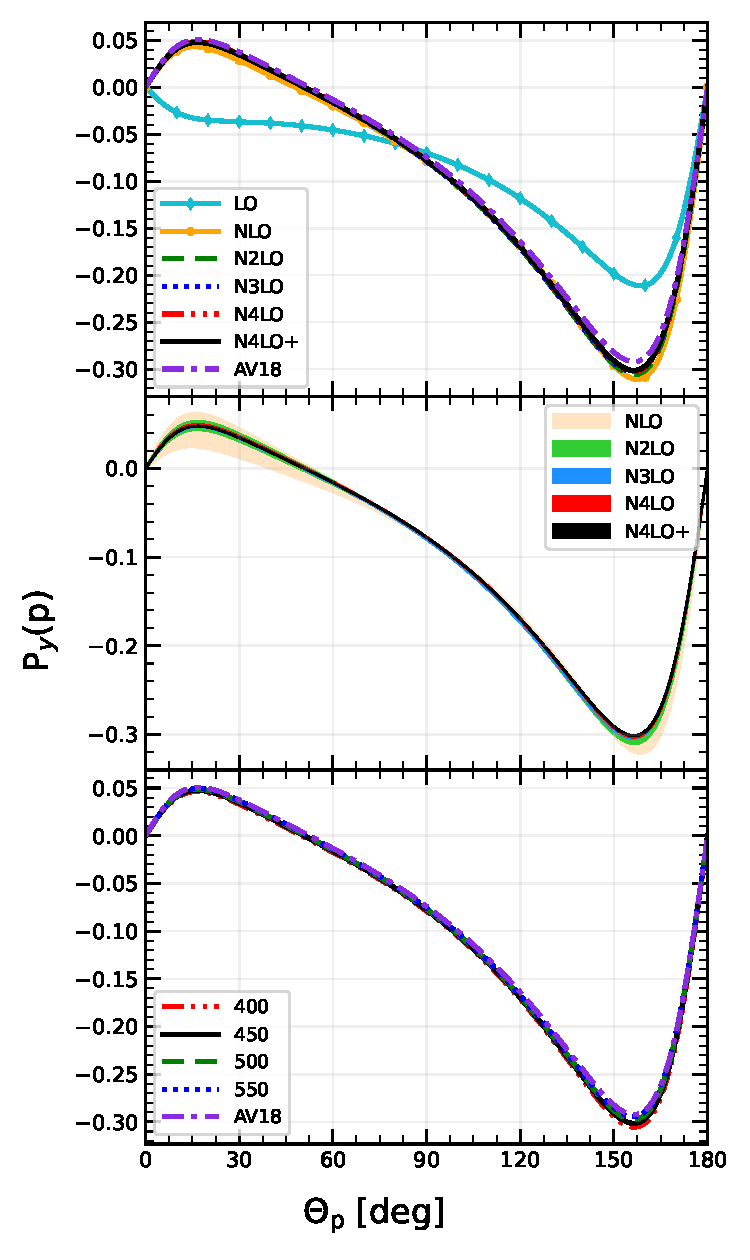
\includegraphics[width=\textwidth]{Figures_De/POLNOUT2(y)_30mev.pdf}
            \caption{\small E$_\gamma = 30$~MeV}
            \label{PY_30_vert}
        \end{subfigure}
        \begin{subfigure}[b]{0.46\textwidth}
            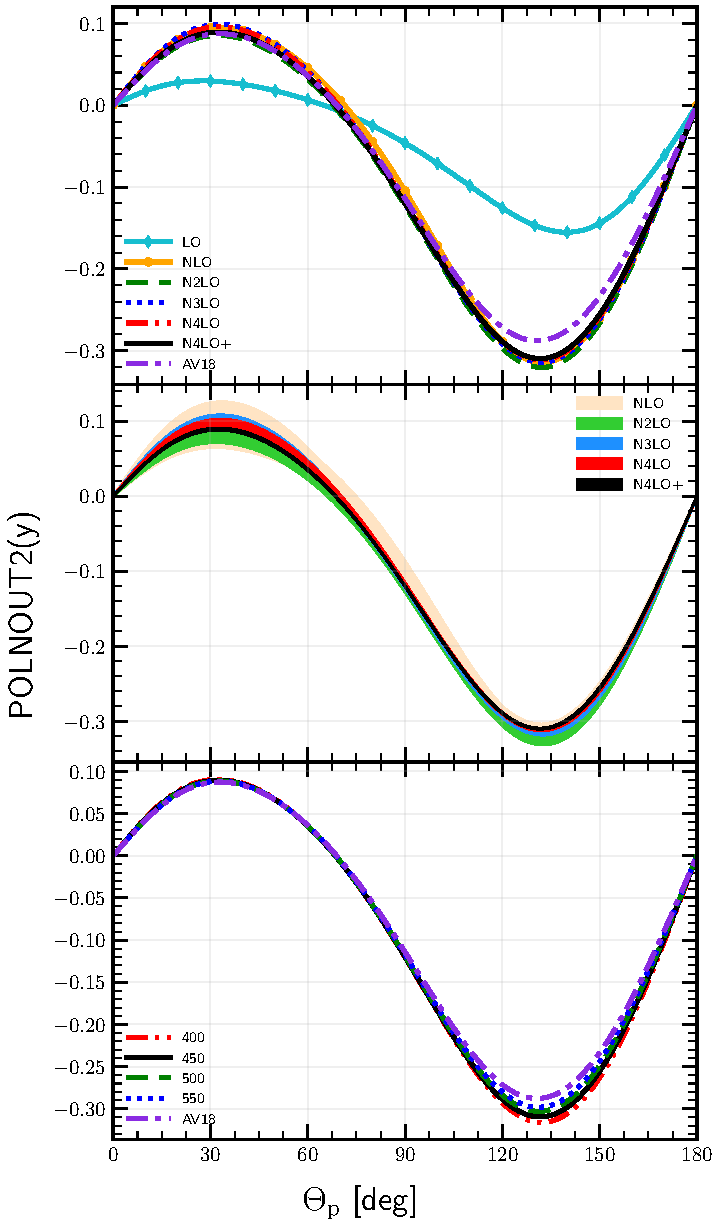
\includegraphics[width=\textwidth]{Figures_De/POLNOUT2(y)_100mev.pdf}
            \caption{\small E$_\gamma = 100$~MeV}
            \label{PY_100_vert}
        \end{subfigure}
        \caption{Proton polarisation $P_y(p)$ 
        \label{PY_30_100_vert}
        as a function of the outgoing proton angle in the center of mass frame 
        for the photon's energy \SI{30}{\mev} (a) and \SI{100}{\mev} (b).
        Top figure presents results obtained using potential
        with different chiral orders (from LO to N$^4$LO+) with cutoff parameter $\Lambda=\SI{450}{\mev}$.
        The middle pane shows truncation errors for each 
        chiral order starting from NLO and
        bottom figure presents a cutoff dependency (chiral potential N$^4$LO+).
        For the sake of comparison, predictions obtained with \gls*{av18} potential are on  figures as well.}
    \end{figure}


    Predictions for the neuteron polarization at energy \SI{2.75}{\mev} and \SI{100}{\mev} are on the
    \fig{Pn_2p75_100}. The choice of energy is conditioned by the availability of experimental data.
    In case of E$_\gamma = \SI{2.75}{\mev}$ (\fig{Pn_2p75_vert}), we can see that predictions reflect
    the behavior of experimental data points qualitatively,
    having more o less constant offset of the values. Similar offset was obtained
    also in predictions at \cite{ArenhovelPhotodisint1991}, where various approaches were presented.
    Interesting is that predictions clearly show symmetrical form of the curve, while in the experimental data
    have some deviations from symmetrical form. It can be a sign that some problem with data can be
    in this case (taking into account also that experiment had been done in 196) as well 
    as inaccuracy in theoretical models.

    At the energy E$_\gamma = \SI{100}{\mev}$ (\fig{Pn_100_vert}), the difference with experimental
    data does not look like a systematic shift and deviations look like random.
    For most of data points, predicted values are within error bars and only some
    of points (e.g. around \ang{50}) have prediction completely out of measured date.
    Nevertheless, whese data points look like being out of general trend an may be
    a result of unpresice measurement.


    \begin{figure}[h]
        % \centering
        % 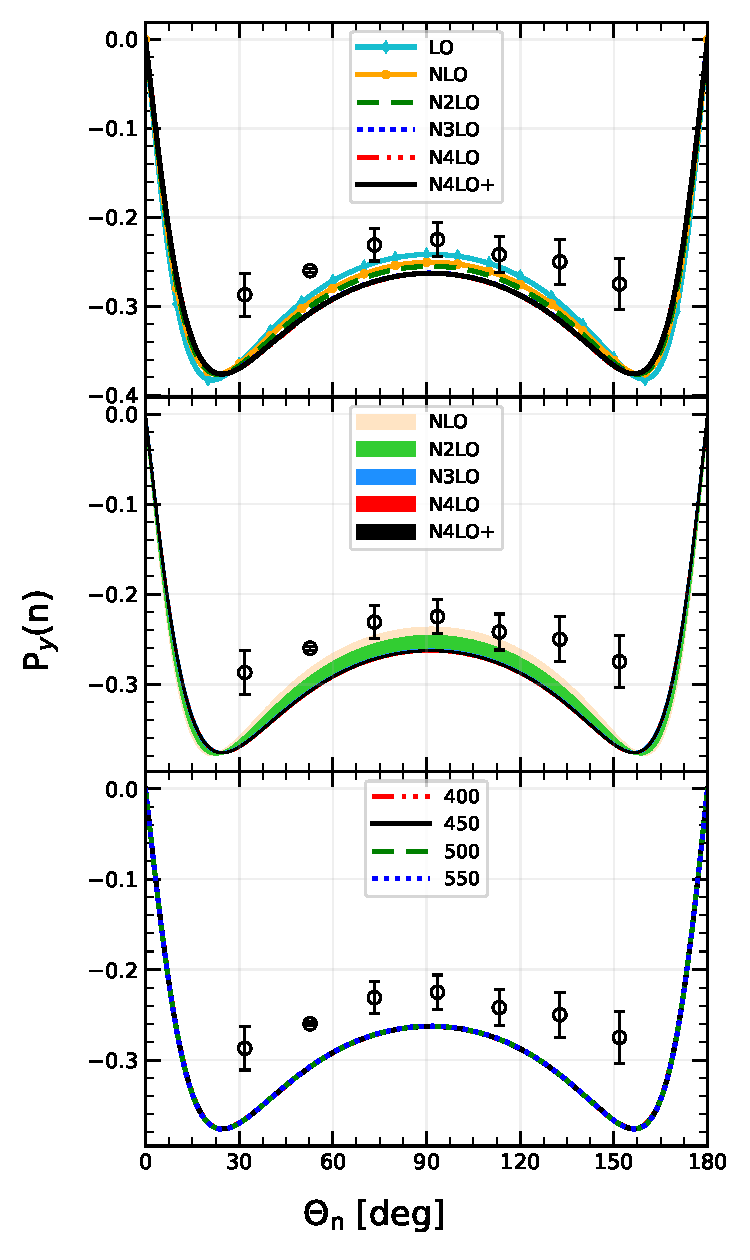
\includegraphics[width=0.5\textwidth]{Figures_De/POLNOUT2(y)_2.75mev_neuteron.pdf}
        \centering
        \begin{subfigure}[b]{0.46\textwidth}
            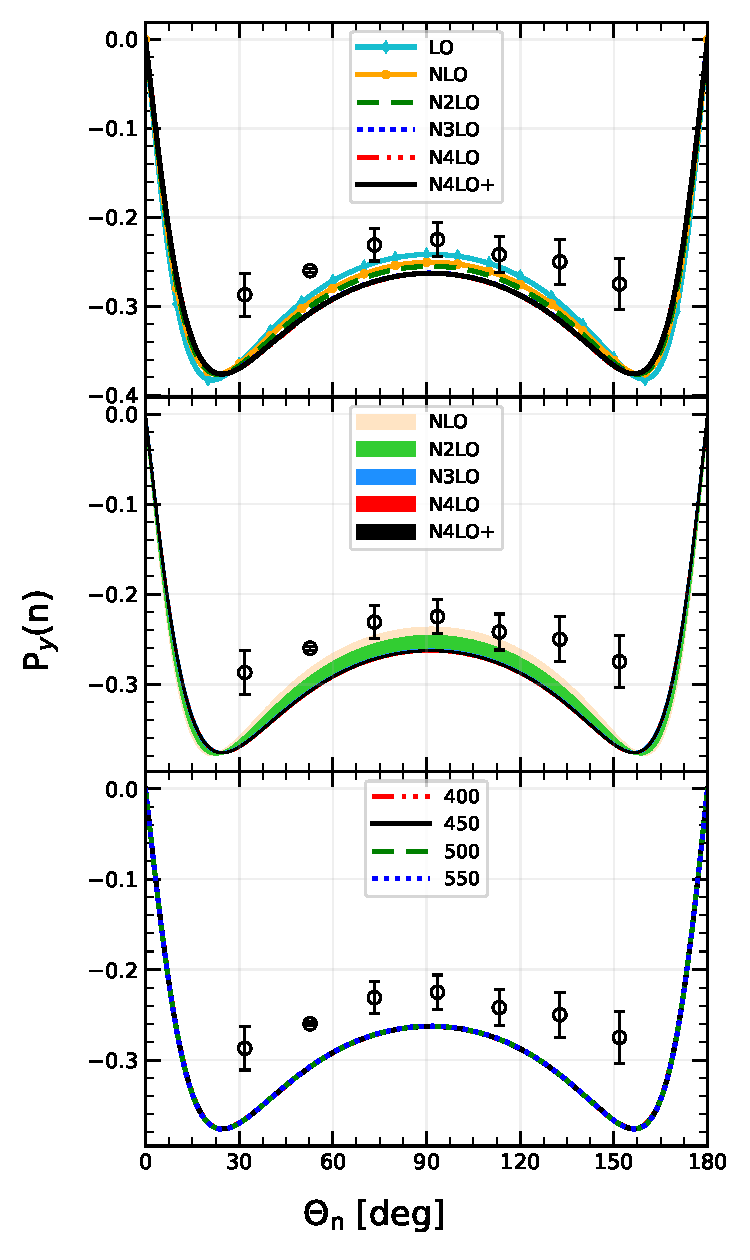
\includegraphics[width=\textwidth]{Figures_De/POLNOUT2(y)_2.75mev_neuteron.pdf}
            \caption{\small E$_\gamma = 2.75$~MeV}
            \label{Pn_2p75_vert}
        \end{subfigure}
        \begin{subfigure}[b]{0.46\textwidth}
            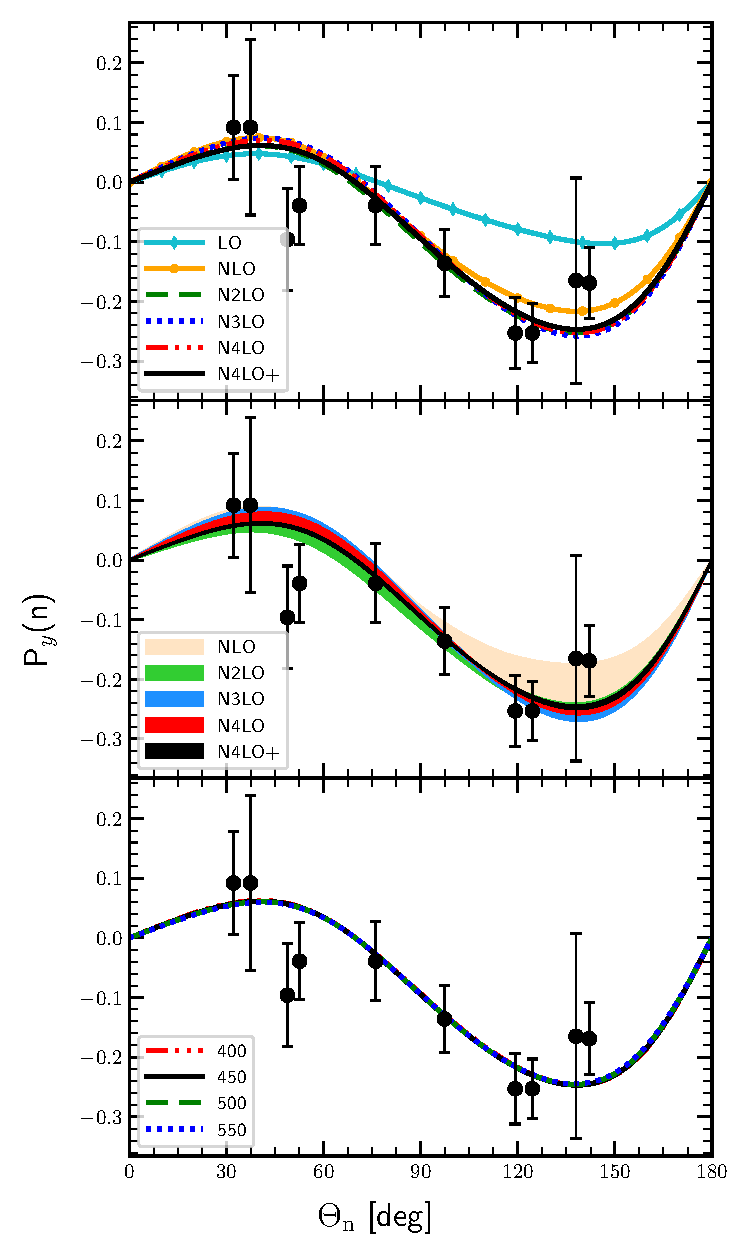
\includegraphics[width=\textwidth]{Figures_De/POLNOUT2(y)_100mev_neuteron.pdf}
            \caption{\small E$_\gamma = 100$~MeV}
            \label{Pn_100_vert}
        \end{subfigure}
        \caption{Neuteron polarisation $P_y(n)$ 
        as a function of the outgoing neuteron angle in the center of mass frame 
        for the photon's energy 2.75 MeV(a) and 100~MeV(b).
        Top row presents results obtained using potential
        with different chiral orders (from LO to N$^4$LO+) with cutoff parameter $\Lambda=\SI{450}{\mev}$.
        The middle pane shows truncation errors for each 
        chiral order starting from NLO and
        bottom figure presents a cutoff dependency (chiral potential N$^4$LO+).
        Experimental data is from \cite{Jewell_neuteronpolarization} (empty circles)
        and \cite{CAMERON_neuteronpolarization} (filled circles).}
        \label{Pn_2p75_100}
    \end{figure}


\clearpage

\section{Helium photodisintegration}
\label{sec:hel_results}

\subsection{3N photodisintegration}

    In this section I will demonstrate predictions
    for observables from $^3\text{He} \rightarrow p + p + n$ process.
    
    On the \fig{CROSS_HE_EXCL_30} I demonstrate a differential cross section 
    $\frac{d^5\sigma}{d\Omega_1d\Omega_2}$ as a function of the S curve position.
    The photon's energy is  E$_\gamma=\SI{30}{\mev}$ and the kinematic configuration
    $\theta_1 = \ang{15}$, $\phi_1 = \ang{0}$,
    $\theta_2 = \ang{15}$, $\phi_2 = \ang{180}$; predictions have been obtained without 3NF.
    We see that only NLO and N$^2$LO introduce relatively large truncation error.
    The maximal width of a band for NLO is \SI{37.6}{\percent} at $S=\SI{10}{\mev}$,
    for N$^2$LO it is \SI{12.4}{\percent} at the same point and it is gradually decreasing
    coming to \SI{0.13}{\percent} at N$^4$LO+.
    The cutoff spread around maxima values is less than \SI{3}{\percent} and it is
    \SI{0.78}{\percent} at the minimum point ($S=\SI{10}{\mev}$).
    

    \begin{figure}[h]
        \begin{center}
            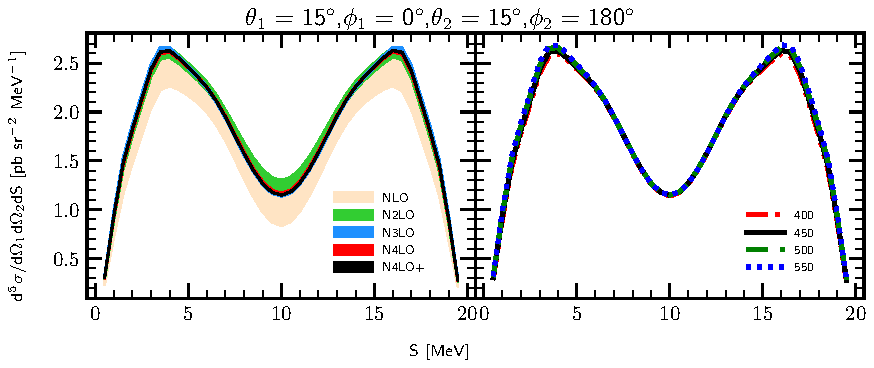
\includegraphics[width=0.9\textwidth]{Figures_HE/CROSS_excl_trunc_30mev.pdf}
            \end{center}
            \caption{The five-fold differential cross section for the photon 
            energy E$_\gamma=\SI{30}{\mev}$ for the kinematic configuration
            $\theta_1 = \ang{15}$, $\phi_1 = \ang{0}$,
            $\theta_2 = \ang{15}$, $\phi_2 = \ang{180}$.
            The left figure presents truncation error bands obtained using potential
            with different chiral orders (from NLO to N$^4$LO+) with
            cutoff parameter $\Lambda=\SI{450}{\mev}$.
            The right figure presents a cutoff dependency (chiral potential N$^4$LO+).
            Results are obtained with two-nucleon force only.}
            \label{CROSS_HE_EXCL_30}
        \end{figure}

    With larger energy E$_\gamma=\SI{100}{\mev}$ demonstrated on the \fig{CROSS_HE_EXCL_100},
    both truncation error and cutoff spread become larger.
    The truncation band at the maximum point $S=\SI{10}{\mev}$ for NLO is \SI{55.0}{\percent}
    decreasing to \SI{2.2}{\percent} at N$^4$LO+ which is around 3 times larger than
    it was in predictions with E$_\gamma=\SI{30}{\mev}$.
    The cutoff spread also becomes larger with increasing energy value: \SI{9.0}{\percent}
    at the same (maximum) point which is also $\sim$3 times larger than the one we observed
    for lower energy.

        \begin{figure}[h]
            \begin{center}
            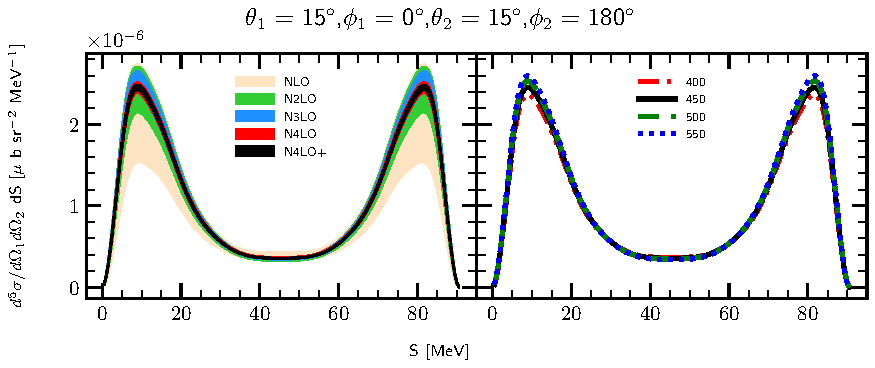
\includegraphics[width=0.9\textwidth]{Figures_HE/CROSS_excl_trunc_100mev.pdf}
            \end{center}
            \caption{The same as on Fig.~\ref{CROSS_HE_EXCL_30} but 
            for the photon energy E$_\gamma=100$~MeV}
            \label{CROSS_HE_EXCL_100}
        \end{figure}

    Next I come to other angular configurations for E$_\gamma=\SI{100}{\mev}$, starting with 
    $\theta_1 = \ang{75}$, $\phi_1 = \ang{75}$,
    $\theta_2 = \ang{75}$, $\phi_2 = \ang{105}$
    demonstrated on \fig{CROSS_HE_EXCL_75_75_75_105}.
    Similar predictions but with 3NF contribution is presented on \fig{CROSS_HE_EXCL_75_75_75_105_3NF}.
    It seems that 3NF does not change much the convergence with respect to the chiral order:
    truncation error band at the point of maximum $S=\SI{35}{\mev}$ (N$^4$LO+)
    is \SI{1.11}{\percent} and \SI{1.16}{\percent} with and without 3NF respectively.
    So it is almost the same, meaning that 3NF contribution does not affect chiral order
    convergence much.

    The cutoff dependence, in turn, is affected by 3NF presence. Predictions with 2NF only have
    \SI{13.7}{\percent} spread at the same maximum point, while predictions with 3NF
    have  \SI{1.23}{\percent}, so the difference is tremendous.

        \begin{figure}[h]
            \begin{center}
                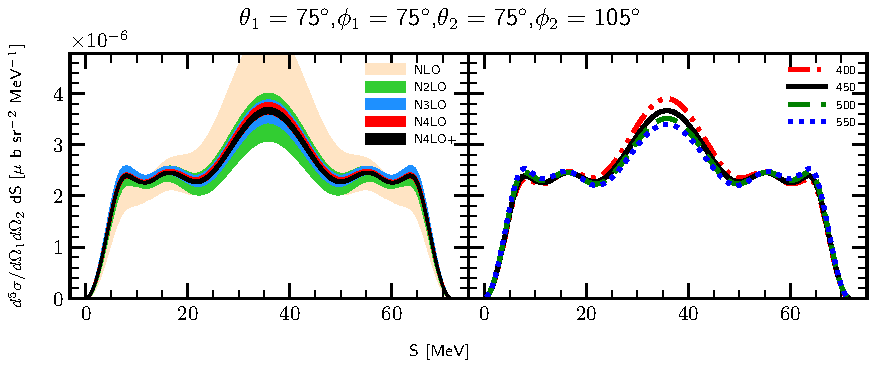
\includegraphics[width=0.9\textwidth]{Figures_HE/CROSS_excl_trunc_100mev_75_75_75_105_2NF.pdf}
                \end{center}
                \caption{The same as on the \fig{CROSS_HE_EXCL_100} but for the different kinematic
                configuration.}
                \label{CROSS_HE_EXCL_75_75_75_105}
        \end{figure}

        \begin{figure}[h]
            \begin{center}
                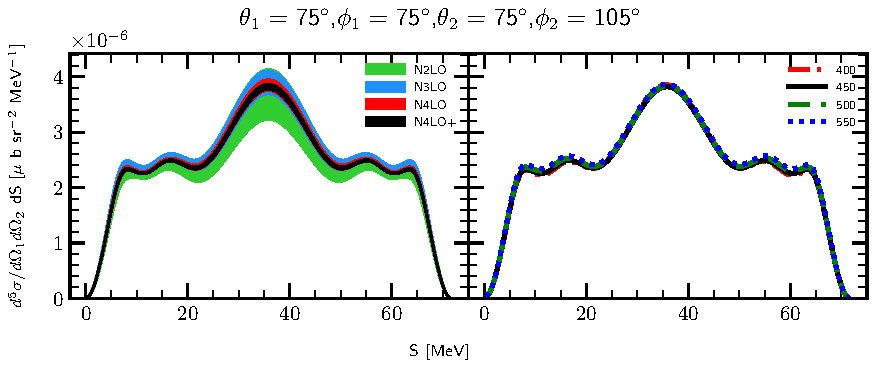
\includegraphics[width=0.9\textwidth]{Figures_HE/CROSS_excl_trunc_100mev_75_75_75_105_3NF.pdf}
                \end{center}
                \caption{The same as on the \fig{CROSS_HE_EXCL_75_75_75_105} but with three-nucleon force.}
                \label{CROSS_HE_EXCL_75_75_75_105_3NF}
        \end{figure}

    Similar trends present in other configurations, demonstrated for the comparison:
    Figs.\ref{CROSS_HE_EXCL_15_105_15_75} and \ref{CROSS_HE_EXCL_15_105_15_75_3NF},
    Figs.\ref{CROSS_HE_EXCL_45_75_45_105} and \ref{CROSS_HE_EXCL_45_75_45_105_3NF},
    Figs.\ref{CROSS_HE_EXCL_165_15_15_165} and \ref{CROSS_HE_EXCL_165_15_15_165_3NF}.

    
        \begin{figure}[h]
            \begin{center}
                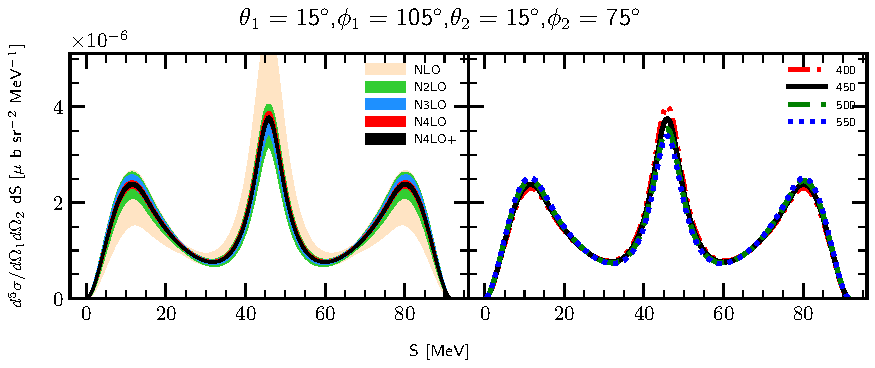
\includegraphics[width=0.9\textwidth]{Figures_HE/CROSS_excl_trunc_100mev_15_105_15_75_2NF.pdf}
                \end{center}
                \caption{The same as on the \fig{CROSS_HE_EXCL_75_75_75_105} but for the different kinematic
                configuration.}
                \label{CROSS_HE_EXCL_15_105_15_75}
        \end{figure}

        \begin{figure}[h]
            \begin{center}
                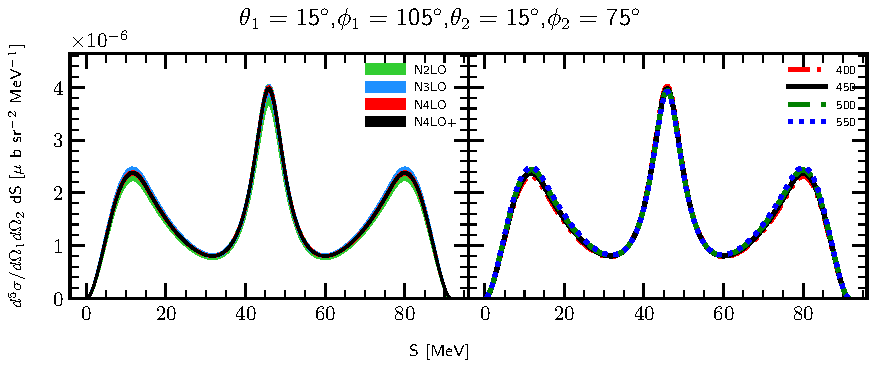
\includegraphics[width=0.9\textwidth]{Figures_HE/CROSS_excl_trunc_100mev_15_105_15_75_3NF.pdf}
                \end{center}
                \caption{The same as on the \fig{CROSS_HE_EXCL_15_105_15_75} but but with three-nucleon force.}
                \label{CROSS_HE_EXCL_15_105_15_75_3NF}
        \end{figure}




        \begin{figure}[h]
            \begin{center}
                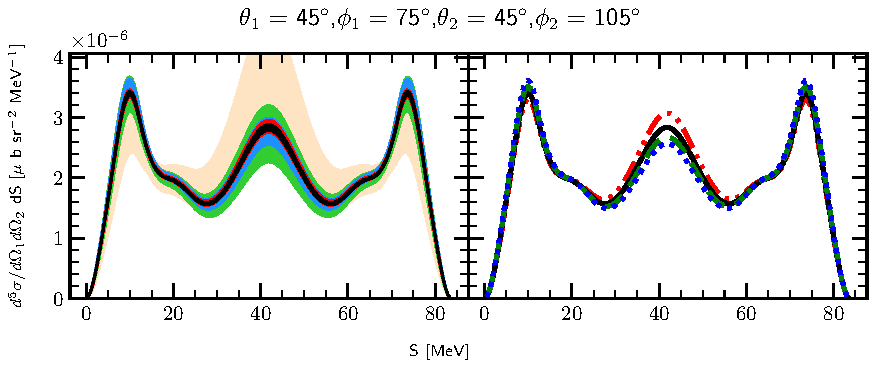
\includegraphics[width=0.9\textwidth]{Figures_HE/CROSS_excl_trunc_100mev_45_75_45_105_2NF.pdf}
                \end{center}
                \caption{The same as on the \fig{CROSS_HE_EXCL_15_105_15_75} but for the different kinematic
                configuration.}
                \label{CROSS_HE_EXCL_45_75_45_105}
        \end{figure}


        \begin{figure}[h]
            \begin{center}
                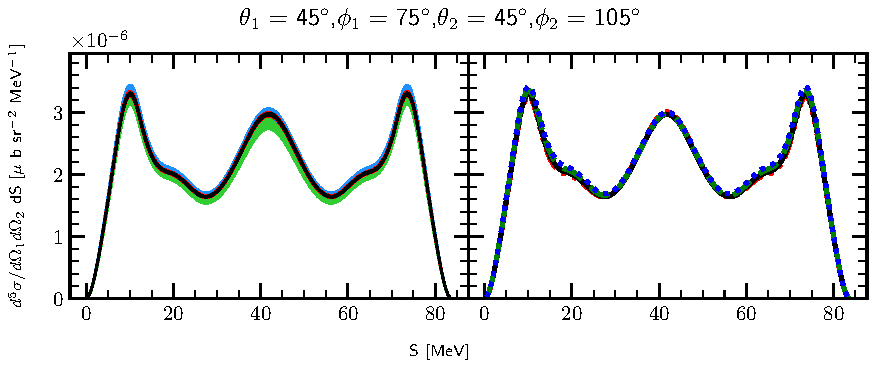
\includegraphics[width=0.9\textwidth]{Figures_HE/CROSS_excl_trunc_100mev_45_75_45_105_3NF.pdf}
                \end{center}
                \caption{The same as on the \fig{CROSS_HE_EXCL_45_75_45_105} but but with three-nucleon force.}
                \label{CROSS_HE_EXCL_45_75_45_105_3NF}
        \end{figure}

        \begin{figure}[h]
            \begin{center}
                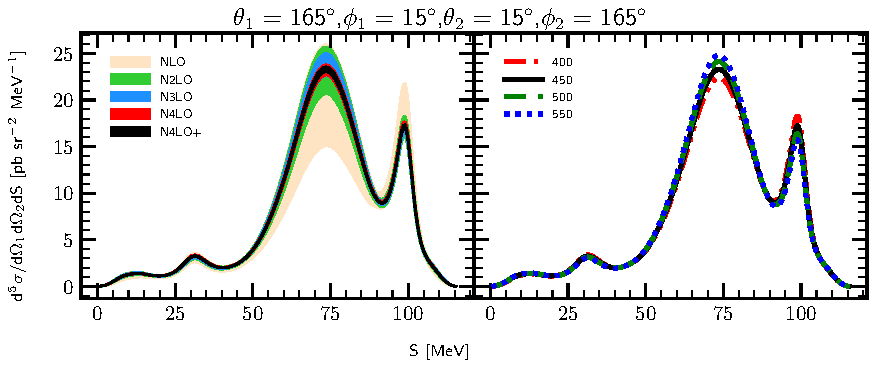
\includegraphics[width=0.9\textwidth]{Figures_HE/CROSS_excl_trunc_100mev_165_15_15_165_2NF.pdf}
                \end{center}
                \caption{The same as on the \fig{CROSS_HE_EXCL_45_75_45_105} but for the different kinematic
                configuration.}
                \label{CROSS_HE_EXCL_165_15_15_165}
        \end{figure}

        \begin{figure}[h]
            \begin{center}
                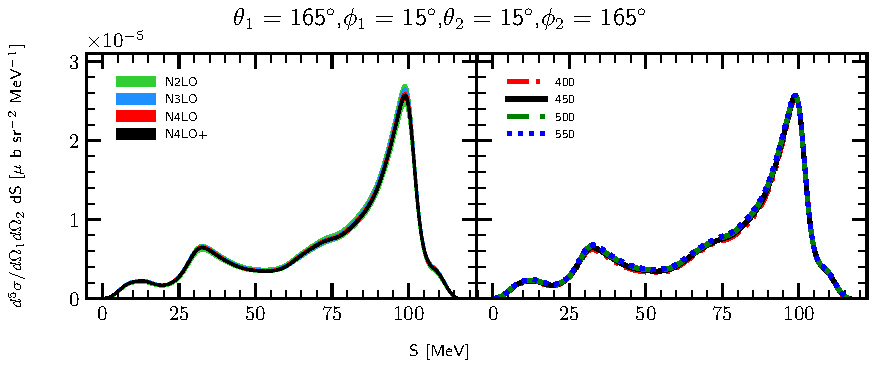
\includegraphics[width=0.9\textwidth]{Figures_HE/CROSS_excl_trunc_100mev_165_15_15_165_3NF.pdf}
                \end{center}
                \caption{The same as on the \fig{CROSS_HE_EXCL_165_15_15_165} but but with three-nucleon force.}
                \label{CROSS_HE_EXCL_165_15_15_165_3NF}
        \end{figure}

        The semi-inclusive differential cross section $\frac{d^3\sigma}{d\Omega_p d\text{E}_p}$
        as a function of the outgoing protons energy $E_p$ is demonstrated on the
        \fig{CROSS_HE_INCL_30MEV_2NF} (for E$_\gamma = \SI{30}{\mev}$) and
        \fig{CROSS_HE_INCL_100MEV_2NF} (for E$_\gamma = \SI{100}{\mev}$).
        Each figure consists of subfigures where each row presents results
        for a proton angles $\theta_p = \ang{10}, \ang{50}, \ang{90}, \ang{130}$ and \ang{170}.
        The left part of each subfigure shows a chiral order dependence while the right - cutoff dependence.
        
        At the photon's energy \SI{30}{\mev} the chiral dependance is relatively weak: at the maximum point
        ($E_p \simeq \SI{3.8}{\mev}$) the relative difference varies between \SI{12}{\percent} and 
        \SI{28}{\percent} at LO for different angles. This difference decreases with each subsequent order
        resulting in \SI{0.15}{\percent} at $N^4LO+$. At the energy $E_\gamma = \SI{100}{\mev}$ truncation errors
        are larger: at the $E_p \simeq \SI{1.46}{\mev}$ the discrepancy is around \SI{40}{\percent} (NLO),
        \SI{15}{\percent} (N2LO), coming to \SI{1.5}{\percent} at N$^4$LO+.

        The cutoff uncertainty at $E_\gamma = \SI{30}{\mev}$ is around \SI{2}{\percent}
        and at $E_\gamma = \SI{100}{\mev}$ is around \SI{8}{\percent} for all angles and 
        at the same values of $E_p$ as regarded above.


        \begin{figure}[h]
            \begin{center}
            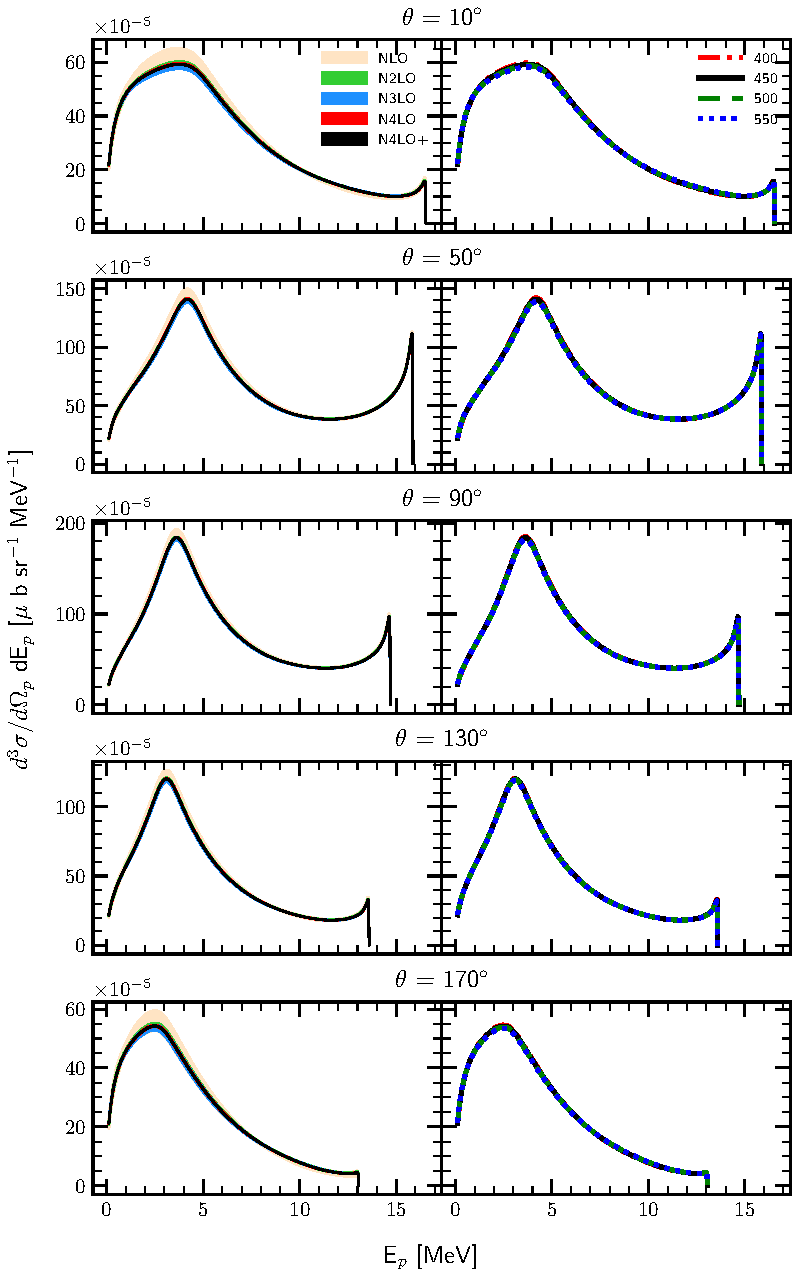
\includegraphics[width=0.8\textwidth]{Figures_HE/CROSS_incl_trunc_30mev_all.pdf}
            \end{center}
            \caption{The semi-inclusive differential cross section $\frac{d^3\sigma}{d\Omega_p d\text{E}_p}$
            at E$_\gamma = \SI{30}{\mev}$ as a function of outgoing proton's energy E$_p$. Each row represent 
            predictions for different values of the outgoing proton's angle $\theta_p$: 
            \ang{10}, \ang{50}, \ang{90}, \ang{130} and \ang{170}. Each column has similar 
            lines and bands definitions as it was for exclusive cross section.  
            Predictions have been obtained without 3NF.}
            \label{CROSS_HE_INCL_30MEV_2NF}
        \end{figure}

        \begin{figure}[h]
            \begin{center}
            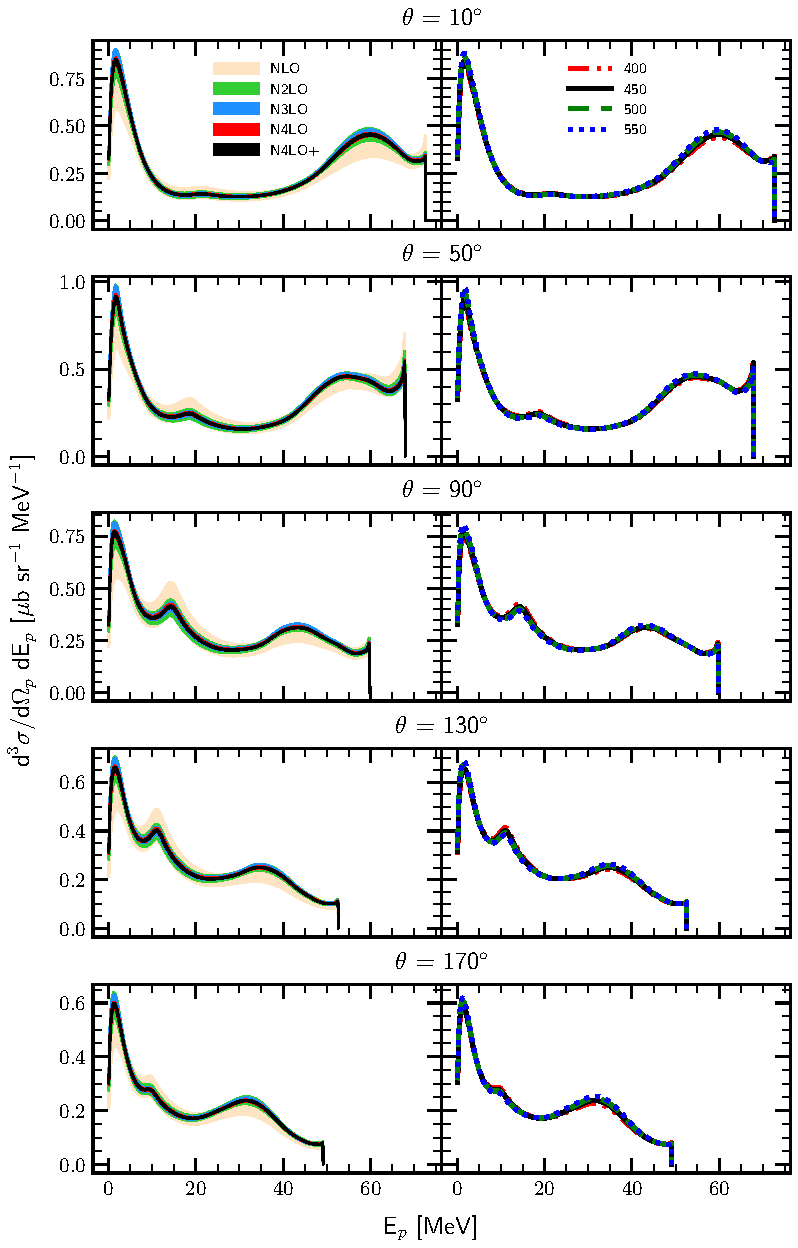
\includegraphics[width=0.8\textwidth]{Figures_HE/CROSS_incl_trunc_100mev_all.pdf}
            \end{center}
            \caption{The same as on \fig{CROSS_HE_INCL_30MEV_2NF} but for E$_\gamma = \SI{100}{\mev}$}
            \label{CROSS_HE_INCL_100MEV_2NF}
        \end{figure}


\clearpage


\subsection{D-n photodisintegration}

    The differential cross section $d\sigma/d\Omega_d$ for the $^3He + \gamma \rightarrow d + n$ reaction
    is presented on the \fig{CROSS_nd_30} (for the photon's energy $E_\gamma = \SI{30}{\mev}$)
    and on the \fig{CROSS_nd_100} (for the photon's energy $E_\gamma = \SI{100}{\mev}$).
    We see that both truncation and cutoff uncertainties are larger with increasing photon's energy.
    The relative spread of the truncation error at the maximum point ($\theta_p = \ang{105}$)
    for the lower energy is \SI{0.05}{\percent} at N$^4$LO+, while for the larger energy
    similar spread is \SI{0.45}{\percent} (at N$^4$LO+, $\theta_p = \ang{120}$).

    The cutoff dependance is also stronger for the larger energy:
    it is  \SI{1.45}{\percent} at \SI{30}{\mev} and \SI{4.01}{\percent} at \SI{100}{\mev}
    (at the points of maximum). 

\begin{figure}[h]
    \begin{center}
        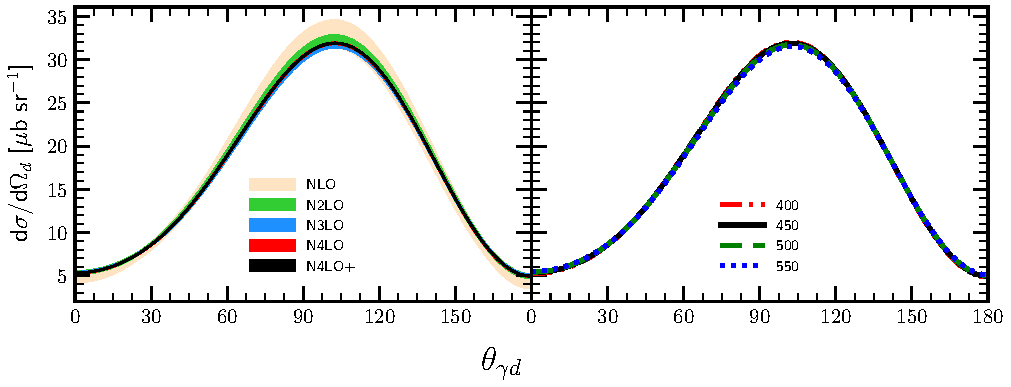
\includegraphics[width=0.9\textwidth]{Figures_HE/CROSS_nd_trunc_30mev.pdf}
        \end{center}
        \caption{Differential cross section for the d-$n$ 
        two-body photodisintegraion of $^3$He as a function of the d$\gamma$ angle.
        The initial photon energy $E_\gamma=\SI{30}{\mev}$.}
        \label{CROSS_nd_30}
    \end{figure}


    \begin{figure}[h]
        \begin{center}
        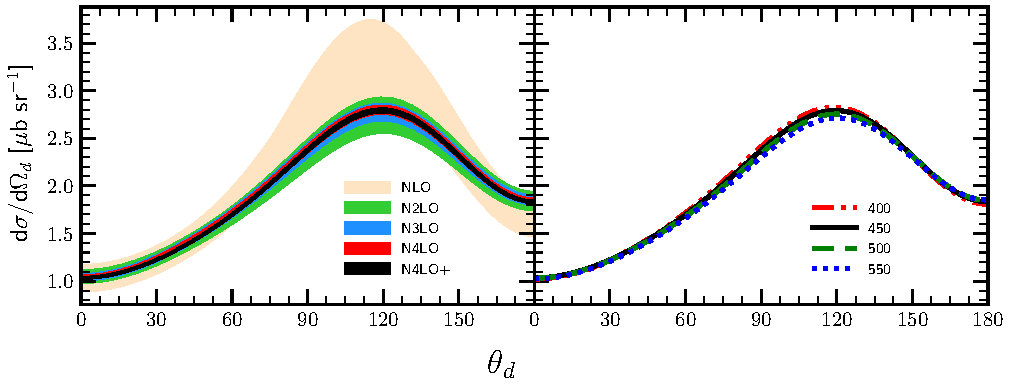
\includegraphics[width=0.9\textwidth]{Figures_HE/CROSS_nd_trunc_100mev.pdf}
        \end{center}
        \caption{The same as on Fig.~\ref{CROSS_nd_30} but 
        for the photon energy E$_\gamma=\SI{100}{\mev}$}
        \label{CROSS_nd_100}
    \end{figure}

    \clearpage

\section{Pion absorption from the lowest atomic orbital}
\label{sec:pion_results}

    \subsection{Pion absorption in $^3$He}

    in \fig{Gamma_pnn} and \ref{Gamma_nd} the pion absorption rates are presented as a functions
    of the chiral order with different values of the cutoff parameter
    (for $\pi^- + ^3He \rightarrow p + n + n$ and $\pi^- + ^3He \rightarrow n + d$ reactions, respectively).
    Both figures show that with fixed chiral order the arrangement of values with respect of the cutoff parameter
    remains the same, namely with increasing $\Lambda$, absorption rate decreases. The only exception in both cases 
    appears at N$^3$LO where prediction with $\Lambda = \SI{550}{\mev}$ goes above other predictions.
    At the next order, N$^4$LO, it corrects to the normal arrangement.
    This behavior may be connected to the 3NF used for the calculation and in order to check that I show
    a similar figure for a proton radius $r_p$ in \fig{proton_rad} calculated with 
    and without 3NF (left and right panels respectively). Results obtained with 3NF show
    similar deviation at N$^3$LO while data obtained without 3NF does not have that.
    Nevertheless, the spread of predictions with respect to the cutoff values is much smaller
    with 3NF and deviation seems to be not crucial as total difference
    between predictions in this case is very small.




    \begin{figure}[h]
        \begin{center}
        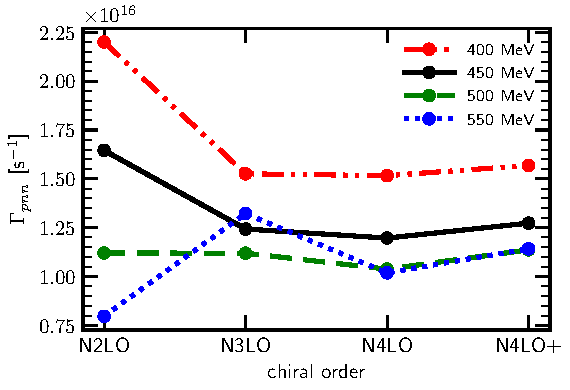
\includegraphics[width=0.6\textwidth]{PlotData/PION/Dalitz_maps/figures/Gamma_pnn.pdf}
        \end{center}
        \caption{Absorption rate for $\pi^- + ^3He \rightarrow p + n + n$ reaction as a function
        of the chiral order with different values of the cutoff parameter $\Lambda$.
        Predictions were obtained with 3NF.}
        \label{Gamma_pnn}
    \end{figure}

    \begin{figure}[h]
        \begin{center}
        \includegraphics[width=0.6\textwidth]{PlotData/PION/Dalitz_maps/figures/Gamma_nd.pdf}
        \end{center}
        \caption{The same as in \fig{Gamma_pnn}, but for $\pi^- + ^3He \rightarrow n + d$ reaction.}
        \label{Gamma_nd}
    \end{figure}

    \begin{figure}[h]
        \begin{center}
        \includegraphics[width=0.99\textwidth]{PlotData/PION/Dalitz_maps/figures/proton_radius_mt31_3NF.pdf}
        \end{center}
        \caption{\tmp{check mt3} Proton radius $r_p$ as a function of the chiral order calculated with
        different values of the cutoff parameter $\Lambda$. The radius was calculated with 2NF and 3NF (left panel)
        and with 2NF only (right panel).}
        \label{proton_rad}
    \end{figure}

    In Figs.~\ref{pion_map_E1E2_cutoff} and \ref{pion_map_xy_cutoff} I show 
    intensity plots for the double differential absorption rates
    $d^2 \Gamma_{pnn}/dE_1dE_2$ for the $\pi^- + ^3He \rightarrow p + n + n$
    process as functions of the nucleons energies (first nucleon is proton) and 
    of \tmp{correct naming} Dalitz coordinates($x$ and $y$) respectively.

    In \fig{pion_map_xy_cutoff} coordinates $x$ and $y$ are defined as:

    \begin{align}
        x &= 3 (E_1 + 2E_2 - E)/E, \nonumber\\
        y &= (3E_1 - E)/E,
        \label{dalitz_xy}
    \end{align}
    taking the region where $r^2 \equiv x^2 + y^2 \leq 1$.

    Each of two figures consists of four panels representing predictions obtained with different 
    values of the cutoff parameter $\Lambda$. The difference between predictions which can be 
    noticed with the naked eye - is that area of the central region (corresponding to smallest values)
    becomes larger with increasing $\Lambda$. It coheres to what we saw on \fig{Gamma_pnn}
    where total absorption rate was inversly correlated with cutoff parameter. The dominant contribution
    comes from the region with lowest proton energy values of $E_1 \rightarrow 0$ where both neutrons have similar large values.
    This is a situation when proton is a spectator while both neutrons share all energy
    - quasi-free scattering(QFS). 

    Another region with high absorption rate is neutron-neutron final state interaction (FSI(nn)).
    It is located at high $E_1$ when proton gets one third part of total energy while neutrons both get
    one sixth.
    
        \begin{figure}[h]
            \begin{center}
            \includegraphics[width=0.7\textwidth]{PlotData/PION/Dalitz_maps/figures/Dalitz_map_pnn_E1E2_cutofs.pdf}
            \end{center}
            \caption{Intensity plots for the double differential absorption rates
            $d^2 \Gamma_{pnn}/dE_1dE_2$ for the $\pi^- + ^3He \rightarrow p + n + n$
            process, obtained using the SMS potential at N$^4$LO+
            with all contributions possible: plane wave + rescattering, SN + 2N, 2NF+3NF.
            Each panel present predictions obtained with different values of the cutoff parameter $\Lambda$:
            from \SI{400}{\mev} (upper left) to \SI{550}{\mev} (lower right). Nucleon 1 is a proton.}
            \label{pion_map_E1E2_cutoff}
        \end{figure}

    \begin{figure}[h]
        \begin{center}
        \includegraphics[width=0.7\textwidth]{PlotData/PION/Dalitz_maps/figures/Dalitz_map_pnn_xy_cutofs.pdf}
        \end{center}
        \caption{The same as in \fig{pion_map_E1E2_cutoff} but for the double differential absorption rates
        $d^2 \Gamma_{pnn}/dxdy$.}
        \label{pion_map_xy_cutoff}
    \end{figure}

    Next I show similar colormaps but for the predictions obtained with plane wave component only (without rescattering part)
    in Figs.~\ref{pion_map_E1E2_cutoff_PW} and \ref{pion_map_xy_cutoff_PW}. Presented plots show that
    the difference of predictions obtained without rescattering part with full is very large. 
    Predicted values 
    are few times larger and the distribution is completely different.
    The FSI(nn) region is not presented here in a sense that there is no peak with respect to other 
    values. The QFS region is, on the contrary, 
    It obviously tells us that one has to take into account rescattering pat in order to obtain relevant results.   

    \begin{figure}[h]
        \begin{center}
        \includegraphics[width=0.7\textwidth]{PlotData/PION/Dalitz_maps/figures/Dalitz_map_pnn_E1E2_cutofs_PWIAS.pdf}
        \end{center}
        \caption{Intensity plots for the double differential absorption rates
        $d^2 \Gamma_{pnn}/dE_1dE_2$ for the $\pi^- + ^3He \rightarrow p + n + n$
        process, obtained using the SMS potential at N$^4$LO+
        with plane wave part only (without rescattering).
        All other contributions are the same as in \fig{pion_map_E1E2_cutoff}: SN + 2N and 2NF+3NF.
        Each panel present predictions obtained with different values of the cutoff parameter $\Lambda$:
        from \SI{400}{\mev} (upper left) to \SI{550}{\mev} (lower right). Nucleon 1 is a proton.}
        \label{pion_map_E1E2_cutoff_PW}
    \end{figure}

    \begin{figure}[h]
        \begin{center}
        \includegraphics[width=0.7\textwidth]{PlotData/PION/Dalitz_maps/figures/Dalitz_map_pnn_xy_cutofs_PWIAS.pdf}
        \end{center}
        \caption{The same as in \fig{pion_map_E1E2_cutoff_PW} but for the double differential absorption rates
        $d^2 \Gamma_{pnn}/dxdy$.}
        \label{pion_map_xy_cutoff_PW}
    \end{figure}

    \begin{figure}[h]
        \begin{center}
        \includegraphics[width=0.7\textwidth]{PlotData/PION/Dalitz_maps/figures/Dalitz_map_pnn_E1E2_cutofs_1NC.pdf}
        \end{center}
        \caption{Intensity plots for the double differential absorption rates
        $d^2 \Gamma_{pnn}/dE_1dE_2$ for the $\pi^- + ^3He \rightarrow p + n + n$
        process, obtained using the SMS potential at N$^4$LO+
        with SN current only (without 2N).
        All other contributions are the same as in \fig{pion_map_E1E2_cutoff}: PWIAS+RESC and 2NF+3NF.
        Each panel present predictions obtained with different values of the cutoff parameter $\Lambda$:
        from \SI{400}{\mev} (upper left) to \SI{550}{\mev} (lower right). Nucleon 1 is a proton.}
        \label{pion_map_E1E2_cutoff_1NC}
    \end{figure}

    \begin{figure}[h]
        \begin{center}
        \includegraphics[width=0.7\textwidth]{PlotData/PION/Dalitz_maps/figures/Dalitz_map_pnn_xy_cutofs_1NC.pdf}
        \end{center}
        \caption{The same as in \fig{pion_map_E1E2_cutoff_1NC} but for the double differential absorption rates
        $d^2 \Gamma_{pnn}/dxdy$.}
        \label{pion_map_xy_cutoff_1NC}
    \end{figure}
    
    \begin{figure}[h]
        \begin{center}
            \includegraphics[width=0.7\textwidth]{PlotData/PION/Dalitz_maps/figures/Dalitz_map_pnn_E1E2_orders.pdf}
        \end{center}
        \caption{Intensity plots for the double differential absorption rates
        $d^2 \Gamma_{pnn}/dE_1dE_2$ for the $\pi^- + ^3He \rightarrow p + n + n$
        process, obtained using the SMS potential at N$^4$LO+
        with all contributions possible: plane wave + rescattering, SN + 2N, 2NF+3NF.
        Each panel present predictions obtained with different chiral orders:
        from N$^2$LO (upper left) to N$^4$LO+ (lower right). Nucleon 1 is a proton.}
        \label{pion_map_E1E2_order}
    \end{figure}

    \begin{figure}[h]
        \begin{center}
        \includegraphics[width=0.7\textwidth]{PlotData/PION/Dalitz_maps/figures/Dalitz_map_pnn_xy_orders.pdf}
        \end{center}
        \caption{The same as in \fig{pion_map_E1E2_order} but for the double differential absorption rates
        $d^2 \Gamma_{pnn}/dxdy$.}
        \label{pion_map_xy_order}
    \end{figure}

    \begin{figure}[h]
        \begin{center}
        \includegraphics[width=0.9\textwidth]{PlotData/PION/Dalitz_maps/figures/3HE_dGdEp.pdf}
        \end{center}
        \caption{}
        \label{pion_GdEp}
    \end{figure}

    \begin{figure}[h]
        \begin{center}
        \includegraphics[width=0.9\textwidth]{PlotData/PION/Dalitz_maps/figures/3HE_dGdEn.pdf}
        \end{center}
        \caption{}
        \label{pion_dGdEn}
    \end{figure}

    \begin{figure}[h]
        \begin{center}
        \includegraphics[width=0.9\textwidth]{PlotData/PION/Dalitz_maps/figures/3HE_dGdr.pdf}
        \end{center}
        \caption{}
        \label{pion_dGdEr}
    \end{figure}

    \begin{figure}[h]
        \begin{center}
        \includegraphics[width=0.9\textwidth]{PlotData/PION/Dalitz_maps/figures/3HE_dGdphi.pdf}
        \end{center}
        \caption{}
        \label{pion_dGdphi}
    \end{figure}


    \clearpage
    \subsection{$\pi^- + ^3$H $\rightarrow n + n + n$}

    \begin{figure}[h]
        \begin{center}
        \includegraphics[width=0.6\textwidth]{PlotData/PION/Dalitz_maps/figures/Gamma_nnn.pdf}
        \end{center}
        \caption{}
        \label{Gamma_nnn}
    \end{figure}


    \begin{figure}[h]
        \begin{center}
        \includegraphics[width=0.7\textwidth]{PlotData/PION/Dalitz_maps/figures/Dalitz_map_nnn_xy_cutofs.pdf}
        \end{center}
        \caption{}
        \label{pion_nnn_xy_cutoff}
    \end{figure}

    \begin{figure}[h]
        \begin{center}
        \includegraphics[width=0.7\textwidth]{PlotData/PION/Dalitz_maps/figures/Dalitz_map_nnn_E1E2_cutofs.pdf}
        \end{center}
        \caption{}
        \label{pion_nnn_E1E2_cutoff}
    \end{figure}

    \begin{figure}[h]
        \begin{center}
        \includegraphics[width=0.7\textwidth]{PlotData/PION/Dalitz_maps/figures/Dalitz_map_nnn_xy_orders.pdf}
        \end{center}
        \caption{}
        \label{pion_nnn_xy_order}
    \end{figure}

    \begin{figure}[h]
        \begin{center}
        \includegraphics[width=0.7\textwidth]{PlotData/PION/Dalitz_maps/figures/Dalitz_map_nnn_E1E2_orders.pdf}
        \end{center}
        \caption{}
        \label{pion_nnn_E1E2_order}
    \end{figure}

    \begin{figure}[h]
        \begin{center}
        \includegraphics[width=0.9\textwidth]{PlotData/PION/Dalitz_maps/figures/3H_dGdEn.pdf}
        \end{center}
        \caption{}
        \label{pion_dGdEn_3H}
    \end{figure}

    \begin{figure}[h]
        \begin{center}
        \includegraphics[width=0.9\textwidth]{PlotData/PION/Dalitz_maps/figures/3H_dGdr.pdf}
        \end{center}
        \caption{}
        \label{pion_dGdr_3H}
    \end{figure}


    \begin{figure}[h]
        \begin{center}
        \includegraphics[width=0.9\textwidth]{PlotData/PION/Dalitz_maps/figures/3H_dGdphi.pdf}
        \end{center}
        \caption{}
        \label{pion_dGdphi_3H}
    \end{figure}
